\documentclass[10pt]{memoir}
\setstocksize{220mm}{155mm} 	        
\settrimmedsize{220mm}{155mm}{*}	
\settypeblocksize{170mm}{116mm}{*}	
\setlrmargins{18mm}{*}{*}
\setulmargins{*}{*}{1.2}
%\setlength{\headheight}{5pt}%
\checkandfixthelayout[lines]
\linespread{1.16}
\flushbottom

%%% Hyphenation settings
\usepackage[htt]{hyphenat}
\hyphenation{he-lio-trope opos-sum}
\tracingparagraphs=1
%Hyphenation in Devanāgarī of the edition still missing? Probably this needs to be modified in babel-iast package? 

%%% babel
\usepackage[english]{babel}
\usepackage{babel-iast/babel-iast}

\babelfont[iast]{rm}[Renderer=Harfbuzz, Scale=1.3]{AdishilaSan}%AdishilaSan}
\babelfont[english]{rm}{Adobe Text Pro}

%%% more functionality
\PassOptionsToPackage{hyphens}{url}
\usepackage{hyperref}
\usepackage{pdflscape}
\usepackage{cleveref}
\usepackage{url}
\usepackage{cleveref}
\usepackage{microtype}
\usepackage{lineno}

%\usepackage{bigfoot}
%%% more functions
\usepackage[dvipsnames]{xcolor}
%\usepackage[para,perpage]{footmisc}

%%%für den Counter von Kapiteln und Sätzen! 
\newcommand{\uproman}[1]{\uppercase\expandafter{\romannumeral#1}}
\newcommand{\lowroman}[1]{\romannumeral#1\relax}

\makeindex
\newfontfamily\sanskritfont[Script=Devanagari,Mapping=RomDev,Scale=1.1]{Sanskrit2003}
\usepackage{pifont,fourier-orns,lettrine,psvectorian,paralist,enumitem,pdfpages,wrapfig,tabulary,lettrine,longtable}
\setlist[enumerate]{itemsep=0mm}
\usepackage[autostyle]{csquotes}
\usepackage[defaultlines=2,all]{nowidow}
\usepackage{ellipsis,adforn,booktabs,longtable,url,tikz}
\lineskiplimit=-3pt          

\makechapterstyle{IeT}{%
  \chapterstyle{default}
  \renewcommand*{\printchapternonum}{\centering}
  \renewcommand*{\clearforchapter}{\cleartorecto} 
  \aliaspagestyle{chapter}{empty}}
\chapterstyle{IeT}
\setsecnumdepth{none}  \openright  \nouppercaseheads
\settocdepth{subsubsection}

%%%% test better pagebreaks
%\def\fussy{%
%  \emergencystretch\z@
%  \tolerance 200%
%  \hfuzz .1\p@
%  \vfuzz\hfuzz}

%\interfootnotelinepenalty=10000\relax

%\usepackage[maxfloats=256]{morefloats}

%\maxdeadcycles=500

%raggedbottomsectiontrue
%%\checkandfixthelayout


%%%%%%%  biblatex
%\newcommand{\noun}[1]{\textsc{#1}}    %  philosophy-verbose
\usepackage[backend=biber, sorting=nyt, style=verbose]{biblatex} %%%%ORIGINAL TiE
\renewcommand*{\mkbibnamefamily}[1]{\textsc{#1}}


\DeclareFieldFormat{url}{%
  \mkbibacro{URL}\addcolon\space
  \href{#1}{\nolinkurl{\thefield{urlraw}}}}

\DeclareFieldFormat{citeurl}{%
  \href{#1}{\nolinkurl{\thefield{urlraw}}}} 


\DeclareFieldFormat{postnote}{#1}
\renewcommand{\postnotedelim}{, }
\addbibresource{bindu.bib}

%%% ekdosis
\usepackage[teiexport=tidy,parnotes=true]{ekdosis}% =tidy cleans up HTML and XML documents by fixing markup errors and upgrading legacy code to modern standards. parnotes=footnotes below or above critical apparatus

\SetLineation{lineation=page, modulo} %lineation=page sets thenumbering to start afresh at the top of each page. =modulo makes every fifth line numbered. {lineation=page} makes every line numbered! 

\renewcommand{\linenumberfont}{\selectlanguage{english}\footnotesize} %sets language of lines to English

\SetTEIxmlExport{autopar=false} %autopar=falseinstructs ekdosis to ignore blank lines in the.tex sourcefile as markers for paragraph boundaries. As a result, each paragraph of the edition must be found within an environment associated with the xml <p> element

\SetHooks{
  lemmastyle=\bfseries,
  %refnumstyle=\selectlanguage{english}\bfseries,
  refnumstyle=\selectlanguage{english}\color{blue}\bfseries,
  appheight=0.8\textheight,
}

\newif\ifinapparatus
\DeclareApparatus{source}[
%bhook=\inapparatustrue,
lang=english,
notelang=english,
% bhook=\selectlanguage{english},
bhook=\selectlanguage{english}\textbf{Sources:},%
%maxentries=4, 
%ehook=.]
%sep={] },
%nosep,
]

\newif\ifinapparatus
\DeclareApparatus{testium}[
%bhook=\inapparatustrue,
lang=english,
notelang=english,
% bhook=\selectlanguage{english},
bhook=\selectlanguage{english}\textbf{Testimonia:},
%maxentries=4, 
%ehook=.]
%nosep, 
]

% Declare \ifinapparatus and set \inapparatustrue at the beginning of
% the apparatus criticus block. Also set the language.  
\newif\ifinapparatus
  \DeclareApparatus{default}[
  %bhook=\inapparatustrue, 
  lang=english,
  %maxentries=33,
  %bhook=\selectlanguage{english},
  sep = {] },
  delim=\hskip 0.75em,
  rule=\rule{0.7in}{0.4pt},
]

\newif\ifinapparatus
\DeclareApparatus{philcomm}[
%bhook=\inapparatustrue,
lang=english,
notelang=english,
bhook=\selectlanguage{english}\textbf{Philological Commentary:},
%bhook=\selectlanguage{english},
sep={: },
]

\ekdsetup{
showpagebreaks,
spbmk = \textcolor{blue}{spb},
hpbmk = \textcolor{red}{hpb}
}

%\usepackage{fnpos}
%\makeFNmid
%\makeFNbottom
\usepackage[bottom]{footmisc}
%%%%%%%%%%%%%%%%%%%%%%%%%%%
\makeatletter
\def\blfootnote{\gdef\@thefnmark{}\@footnotetext}
\makeatother
%%%%%%%%%%%%%%%%%%%%%%%%%


% Macros and Definitions for the Print of Sigla
\def\acpc#1#2#3{{#1}\rlap{\textrm{\textsuperscript{#3}}}\textsubscript{\textrm{#2}}\space}
\def\sigl#1#2{{{#1}}\textsubscript{\textrm{#2}}}
\def\None{{\sigl{N}{1}}} \def\Noneac{\acpc{N}{1}{ac}\,} \def\Nonepc{\acpc{N}{1}{pc}\,}
\def\Ntwo{{\sigl{N}{2}}} \def\Noneac{\acpc{N}{2}{ac}\,} \def\Nonepc{\acpc{N}{2}{pc}\,}
\def\Done{{\sigl{D}{1}}} \def\Doneac{\acpc{D}{1}{ac}\,} \def\Donepc{\acpc{D}{1}{pc}\,}
\def\Dtwo{{\sigl{D}{2}}} \def\Dtwoac{\acpc{D}{2}{ac}\,} \def\Dtwopc{\acpc{D}{2}{pc}\,}
\def\Uone{{\sigl{U}{1}}} \def\Uoneac{\acpc{U}{1}{ac}\,} \def\Uonepc{\acpc{U}{1}{pc}\,}                 
\def\Utwo{{\sigl{U}{2}}} \def\Utwoac{\acpc{U}{2}{ac}\,} \def\Utwopc{\acpc{U}{2}{pc}\,}

%%%%%%%%%%%%%% Tattvabinduyoga - List of Witnesses   %%%%%%%%%%%%%%%%%%%
\DeclareWitness{ceteri}{\selectlanguage{english}cett.}{ceteri}[]   
\DeclareWitness{E}{\selectlanguage{english}E}{Printed Edition}[]    
\DeclareWitness{P}{\selectlanguage{english}P}{Pune BORI 664}[]  
\DeclareWitness{B}{\selectlanguage{english}B}{Bodleian 485}[]       
\DeclareWitness{N1}{\selectlanguage{english}N\textsubscript{1}}{NGMPP 38/31}[]
\DeclareWitness{N2}{\selectlanguage{english}N\textsubscript{2}}{NGMPP B 38/35}[]
\DeclareWitness{L}{\selectlanguage{english}L}{LALCHAND 5876}[]  
\DeclareWitness{D}{\selectlanguage{english}D}{IGNCA 30019}[] 
%\DeclareWitness{D2}{\selectlanguage{english}D\textsubscript{2}}{IGNCA 30020}[]  
\DeclareWitness{U1}{\selectlanguage{english}U\textsubscript{1}}{SORI 1574}[] 
\DeclareWitness{U2}{\selectlanguage{english}U\textsubscript{2}}{SORI 6082}[]
%%%%%%%%%%%%%% Tattvabinduyoga - Groups of Witnesses   %%%%%%%%%%%%%%%%%%%
\DeclareWitness{X}{\selectlanguage{english}\alpha}{Alpha Group: D,N1,N2,U1}[]
\DeclareWitness{Y}{\selectlanguage{english}\beta}{Beta Group: B,E,L,P,U2}[]
%%%%%%%%%%%%% Testimonia
\DeclareWitness{Ysv}{\selectlanguage{english}Ysv}{Yogasvarodaya}[] %%%add infos!  

%%%%%%%%%%%%%%%%%%%%%%%%%%%%%%%%%%%%%%%%%%%
% Macro for Editing Abbrevs.
\def\om{\textrm{\footnotesize \textit{om.}\ }} %prints om. for omitted in apparatus
\def\korr{\textrm{\footnotesize \textit{em.}\ }} %prints em. for emended in apparatus
\def\conj{\textrm{\footnotesize \textit{conj.}\ }} %prints conj. for conjectured in apparatus

% \supplied{text} EDITORIAL ADDITION -> Within \lem oder \rdg
% \surplus{text} EDITORIAL DELETION -> Within \lem oder \rdg
% \sic{text} CRUX
% \gap{text} LACUNAE -> [reason=??, unit=??, quantity=??, extent=??]


%%%%%%%%%%%%%%%%%%%%%%%%%%%%%%%%%%%%%%%%%%% All macros of this list can be used in 
% Macro for Editing Abbrevs.
\def\eyeskip{\textrm{{ab.\,oc. }}}
\def\aberratio{\textrm{{ab.\,oc. }}}
\def\ad{\textrm{{ad}}}
\def\add{\textrm{{add.\ }}}
\def\ann{\textrm{{ann.\ }}}
\def\ante{\textrm{{ante }}} 
\def\post{\textrm{{post }}}
%\def\ceteri{cett.\,}                   
\def\codd{\textrm{{codd.\ }}}

\def\coni{\textrm{{coni.\ }}}
\def\contin{\textrm{{contin.\ }}}
\def\corr{\textrm{{corr.\ }}}
\def\del{\textrm{{del.\ }}}
\def\dub{\textrm{{ dub.\ }}}

\def\expl{\textrm{{explic.\ }}} 
\def\explica t{\textrm{{explic.\ }}}
\def\fol{\textrm{{fol.\ }}}
\def\foll{\textrm{{foll.\ }}}
\def\gloss{\textrm{{glossa ad }}}
\def\ins{\textrm{{ins.\ }}}      
\def\inseruit{\textrm{{ins.\ }}} 
\def\im{{\kern-.7pt\lower-1ex\hbox{\textrm{\tiny{\emph{i.m.}}}\kern0pt}}} %\textrm{\scriptsize{i.m.\ }}}      
\def\inmargine{{\kern-.7pt\lower-.7ex\hbox{\textrm{\tiny{\emph{i.m.}}}\kern0pt}}}%\textrm{\scriptsize{i.m.\ }}}      
\def\intextu{{\kern-.7pt\lower-.95ex\hbox{\textrm{\tiny{\emph{i.t.}}}\kern0pt}}}%\textrm{\scriptsize{i.t.\ }}}           
\def\indist{\textrm{{indis.\ }}}  
\def\indis{\textrm{{indis.\ }}}
\def\iteravit{\textrm{{iter.\ }}} 
\def\iter{\textrm{{iter.\ }}}
\def\lectio{\textrm{{lect.\ }}}   
\def\lec{\textrm{{lect.\ }}}
\def\leginequit{\textrm{{l.n. }}} 
\def\legn{\textrm{{l.n. }}}
\def\illeg{\textrm{{l.n. }}}

\def\primman{\textrm{{pr.m.}}}
\def\prob{\textrm{{prob.}}}
\def\rep{\textrm{{repetitio }}}
\def\secundamanu{\textrm{\scriptsize{s.m.}}}            \def\secm{{\kern-.6pt\lower-.91ex\hbox{\textrm{\tiny{\emph{s.m.}}}\kern0pt}}}%   \textrm{\scriptsize{s.m.}}}
\def\sequentia{\textrm{{seq.\,inv.\ }}}  
\def\seqinv{\textrm{{seq.\,inv.\ }}}
\def\order{\textrm{{seq.\,inv.\ }}}
\def\supralineam{{\kern-.7pt\lower-.91ex\hbox{\textrm{\tiny{\emph{s.l.}}}\kern0pt}}} %\textrm{\scriptsize{s.l.}}}
\def\interlineam{{\kern-.7pt\lower-.91ex\hbox{\textrm{\tiny{\emph{s.l.}}}\kern0pt}}}   %\textrm{\scriptsize{s.l.}}}
\def\vl{\textrm{v.l.}}   \def\varlec{\textrm{v.l.}} \def\varialectio{\textrm{v.l.}}
\def\vide{\textrm{{cf.\ }}}
\def\cf{\textrm{{cf.\ }}} 
\def\videtur{\textrm{{vid.\,ut}}}
\def\crux{\textup{[\ldots]} }
\def\cruxx{\textup{[\ldots]}}
\def\unm{\textit{unm.}}
%%%%%%%%%%%%%%%%%%%%%%%%%%%%%%%%%%%%

% List of Scholars
\DeclareScholar{ego}{ego}[
forename=Nils Jacob,
surname=Liersch]

% Persons:14\DeclareScholar{ego}{ego}[15forename=Robert,16surname=Alessi]17% Useful shorthands:18\DeclareShorthand{codd}{codd.}{V,I,R,H}19\DeclareShorthand{edd}{edd.}{Lit,Erm,Sm}20\DeclareShorthand{egoscr}{\emph{scripsi}}{ego}

%Useful shorthands:
%\DeclareShorthand{codd}{codd.}{V,I,R,H}
%\DeclareShorthand{edd}{edd.}{Lit,Erm,Sm}
\DeclareShorthand{egoscr}{em.}{ego}
\DeclareShorthand{egoscrconj}{conj.}{ego}
\DeclareShorthand{egomute}{\unskip}{ego}

\usepackage{xparse}

\NewDocumentEnvironment{tlg}{O{}O{}}{\setlength{\leftskip}{0pt}\vspace{-1ex}\begin{quotation}}{\hfill #1\ \vspace{-1ex}\end{quotation}\vspace{-1ex}} %verse environment
%\NewDocumentEnvironment{tlg}{O{}O{}}{\begin{verse}}{॥#1\hskip-4pt ॥\\ \end{verse}}
\NewDocumentCommand{\tl}{m}{{\selectlanguage{iast} #1}}

\NewDocumentCommand{\extra}{m}{{\textcolor{gray}{#1}}} %command for additions to U2
\NewDocumentCommand{\crazy}{m}{{\textcolor{red}{#1}}} %totally corrupted passage
\NewDocumentCommand{\coro}{m}{{\textcolor{violet}{#1}}} %colour for sentence counter! 

\NewDocumentEnvironment{prose}{O{}}{\begin{otherlanguage}{iast}}{\end{otherlanguage}}
% \NewDocumentEnvironment{padd}{O{}}{\begin{otherlanguage}{iast}}{\end{otherlanguage}}
\NewDocumentEnvironment{tlate}{O{}}
%\NewDocumentEnvironment{tadd}{O{}}

%Define two commands: \skp ("sanskrit plus"), to be ignored by TeX in
%the edition text, but processed in the TEI output. Conversely, \skm
%("sanskrit minus") is to be processed in the edition text, but
%ignored if found in the apparatus criticus and in the TEI output:

\NewDocumentCommand{\skp}{m}{}
\TeXtoTEIPat{\skp {#1}}{#1}

%\NewDocumentCommand{\skpp}{m}{}
%\TeXtoTEIPat{\skpp {#1}}{#1}

\NewDocumentCommand{\skm}{m}{\unless\ifinapparatus#1-\fi}
\TeXtoTEIPat{\skm {#1}}{}

% \NewDocumentCommand{\dd}{}{/\hskip-4pt/}
\NewDocumentCommand{\dd}{}{\mbox{/\hskip-4pt/}}
\TeXtoTEIPat{\dd {}}{//}


%%% modify environments and commands
%%% TEI mapping
\TeXtoTEIPat{\begin {tlg}}{<lg>} %lg=(Group of verse (s)) contains one or more verses or lines of verse that together form a formal unit (e.g. stanza, chorus).
\TeXtoTEIPat{\end {tlg}}{</lg>}

\TeXtoTEIPat{\begin {prose}}{<p>}
\TeXtoTEIPat{\end {prose}}{</p>}

\TeXtoTEIPat{\begin {tlate}}{<p>}
\TeXtoTEIPat{\end {tlate}}{</p>}

\TeXtoTEIPat{\\}{}
\TeXtoTEIPat{\linebreak}{<br/>}
\TeXtoTEIPat{\noindent}{}
%\TeXtoTEI{tl}{l}
\TeXtoTEI{emph}{hi}
\TeXtoTEI{bigskip}{}
\TeXtoTEI{None}{N1}
\TeXtoTEI{Ntwo}{N2}
\TeXtoTEI{Done}{D1}
\TeXtoTEI{Dtwo}{D2}
\TeXtoTEI{Uone}{U1}
\TeXtoTEI{Utwo}{U2}
%\TeXtoTEIPat{/}{ |}
%\TeXtoTEI{//}{ ||}
\TeXtoTEIPat{\korr}{em. }
\TeXtoTEIPat{\conj}{conj.}
\TeXtoTEIPat{\om}{om.}
\TeXtoTEIPat{english}{}
\TeXtoTEIPat{\hskip}{}
\TeXtoTEIPat{\hskip-4pt}{}
\TeXtoTEIPat{\hskip-2pt}{}
\TeXtoTEIPat{-}{ }
\TeXtoTEIPat{4pt}{}
\TeXtoTEIPat{2pt}{}
\TeXtoTEIPat{\textcolor {#1}{#2}}{<hi rend="#1">#2</hi>} 

% Nullify \selectlanguage in TEI as it has been used in
% \DeclareWitness but should be ignored in TEI.
\TeXtoTEI{selectlanguage}{}



\FormatDiv{1}{\begin{center}\Large}{\end{center}}
\FormatDiv{2}{\begin{center}\small}{\end{center}}
\FormatDiv{3}{\bfseries}{.}
\title{Yogatattvabindu of Rāmacandra\\ A Critical Edition and Annotated Translation}
\date{\today}

\parindent=15pt
\begin{document}

% Zitiermöglichkeiten:
%\footcite[See][p.\,1]{goldstein01:_tibet_englis_diction_moder_tibet}
%\footnote{\cite{goldstein01:_tibet_englis_diction_moder_tibet}.}

\frontmatter
\thispagestyle{empty}
\begin{center}
  {\Large \emph{The Yogatattvabindu}}\\[3mm]
\end{center}



\newpage

\

\thispagestyle{empty}



\normalsize


\newpage


\begin{center}
\thispagestyle{empty}

\

\vskip 2mm

\begin{otherlanguage}{iast}
\LARGE \sanskritfont{Yogatattvabindu}
\end{otherlanguage}

\vskip .4cm

\Huge Yogatattvabindu \\[7mm]
\Large Critical Edition\\
with annotated Translation


\large

\vspace{3cm}

Von

Nils Jacob Liersch
\small
\vfill

\vfill

Indica et Tibetica Verlag \\ % $\cdot$ 
Marburg 2024

\vskip 6mm

\end{center}

\newpage
\newpage \ \thispagestyle{empty}
\small  \

\noindent

\
\vfill


\small
\noindent \textbf{Bibliographische Information Der Deutschen Bibliothek}

\noindent
Die Deutsche Bibliothek verzeichnet diese Publikation in der Deutschen Nationalbibliographie;
detaillierte bibliographische Informationen sind im Internet über http://dnb.ddb.de abrufbar.

\noindent
\textbf{Bibliographic information published by Die Deutschen Bibliothek}

\noindent
Die Deutsche Bibliothek lists this publication in the Deutsche Nationalbibliographie; detailed
bibliographic data is available in the Internet at http://dnb.ddb.de.  


\vskip 1cm

\noindent
\copyright\ Indica et Tibetica Verlag, Marburg 2024

\medskip

\noindent
Alle Rechte vorbehalten / All rights reserved

\medskip

\noindent
Ohne ausdrückliche Genehmigung des Verlages ist es nicht gestattet, das Werk oder einzelne Teile
daraus nachzudrucken, zu vervielfältigen oder auf Datenträger zu speichern.

\smallskip

\noindent
Apart from any fair dealing for the purpose of private study, research, criticism or review, no
part of this book may be reproduced or translated in any form, by print, photo form, microfilm, or
any other means without written permission. Enquiries should be made to the publishers.

\bigskip

\noindent
Satz: \ \ Nils Jacob Liersch \\
Herstellung: \ \ BoD – Books on Demand GmbH, Norderstedt  \\

\bigskip

\noindent
%\ISBN     

\normalsize

\newpage

%\maketitle
\clearpage
\tableofcontents
\addtocounter{page}{-1}
\thispagestyle{empty}
\clearpage


\mainmatter

\chapter{Conventions in the Critical Apparatus}
\section{Sigla in the Critical Apparatus}

\begin{itemize}
\item E : Printed Edition
\item P : Pune BORI 664
\item L : Lalchand Research Library LRL5876
\item B : Bodleian Oxford D 4587
\item \None : NGMPP B 38-31
\item \Ntwo : NGMPP B 38-35 / A 1327-14
\item \Done : IGNCA 30019
\item \Uone : SORI 1574
\item \Utwo: SORI 6082
\end{itemize}

\chapter{Critical Edition \& Annotated Translation}
\cleardoublepage
\begin{alignment}[
  texts=edition[class="edition"];
  translation[class="translation"],
  ]
  \begin{edition}
                   \ekddiv{
                     head={[\uproman{16}. \textbf{rājayogayuktasya puruṣasya yac charīracihnam}]},
                     type=section,
                     depth=2, 
                     n=XVI
                   }
           \xmlhead[h16]{[XVI. rājayogayuktasya puruṣasya yac charīracihnam]}
                  \label{rajabody}
                      \begin{prose}[p16_01]
      \noindent
%------------------------------  
%idānīṃ rājayogayuktasya           śarīre yaccihnaṃ  tat    kathyate / \E
%idānīṃ rājayogayuktasya puruṣasya yaccharīracihnaṃ         kathyate / \P
%idānīṃ rājayogayuktasya puruṣasya          cinhnaṃ         kathyate / \L
%idānīṃ rājayogayuktasya puruṣasya          cinhnaṃ         kathyate // \B
%idānīṃ rājayogayuktasya puruṣasya yaccarīracihnaṃ   tat    kathyate / \N1
%idānīṃ rājayogayuktasya puruṣasya yaccharīracihūṃ   tat    kathyate// \N2
%idānīṃ rājayogayuktasya puruṣasya yaccarīracihnaṃ   tat    kathyate / \D
%idānīṃ rājayogayuktasya puruṣasya yaccharīre cinhaṃ tata   kathyate \U1
%idānīṃ rājayogayuktasya puruṣasya yat śarīracinhaṃ         kathyate / \U2
%------------------------------
%Now, the sign of the body of the person who is endowed with Rājayoga is taught.
%------------------------------
\note[type=philcomm, labelb=_117ab, labele={_117x}, lem={idānīṃ rājayogayuktasya puruṣasya yaccarīracihnaṃ \ldots sthāne'nurāgaṃ na prāpnoti}]{This whole section of the text contains several omissions of complete sentences. Due to their brevity and the similarity in structure, various writers might have inadvertently caused these omissions due to eye-skipping.}      
\note[type=source, labelb=_117ab, labele={_117c}, nosep]{cf. YSv (PT p. 834): idānīṃ kathayiṣyāmi rājayogasya lakṣaṇam | rājayoge kṛte puṃbhiḥ siddhicihnaṃ bhaved iti |}
      idānīṃ rājayogayuktasya
  \app{\lem[wit={ceteri}]{puruṣasya}
    \rdg[wit={E}]{\om}}
  \app{\lem[wit={D,N1,P},alt={yac charīracihnaṃ}]{yac-charīracihnaṃ}
    \rdg[wit={B,L}]{cinhnaṃ}
    \rdg[wit={E}]{śarīre yac cihnaṃ}
    \rdg[wit={U1}]{yac charīre cinhaṃ}
    \rdg[wit={U2}]{yat śarīracinhaṃ}  
    \rdg[wit={N2}]{yac charīracihūṃ}
    }
  \app{\lem[wit={D,E,N1,N2}]{tat}
    \rdg[wit={U1}]{tata}
    \rdg[wit={ceteri}]{\om}} kathyate/
%------------------------------  
%tatsarvatra pūrṇo bhavati / \E
%tatsarvatra pūrṇā bhavati / \P
%tatsarvatra pūrṇo bhavati / \L
%tatsarvatra pūrṇo bhavatī / \B
%  sarvvatra pūrṇo bhavati / \N1
%  sarvvatra pūrṇā bhavati  \N2
%  sarvvatra pūrṇo bhavati  \D
%  sarvvatra pūrṇo bhavati   \U1
%tatsarvatra pūrṇo bhavati// \U2
%------------------------------
%Abundance arises at all times.    
%------------------------------
\note[type=source, labelb=117, nosep]{cf. YSv (PT p. 834): paripūrṇaṃ bhavec cittaṃ jagatstho'pi jagadbahiḥ |}
  \app{\lem[wit={X},alt={sarvatra°}]{sarvatra}
  \rdg[wit={Y}]{tatsarvatra°}}
\app{\lem[wit={ceteri}, alt={°pūrṇo}]{pūrṇo}
  \rdg[wit={P,N2}]{pūrṇā}}
\app{\lem[wit={ceteri}]{bhavati}
  \rdg[wit={B}]{bhavatī}}/
%------------------------------  
%pṛthivyāḥ dūre tiṣṭhati / \E
%pṛthivyāḥ hare tiṣṭhati / \P
%\om                      \L
%\om                      \B
%pṛthivyāḥ dūre  tiṣṭhati / \N1
%pṛthivyāḥ dūra  tiṣṭhati / \N2
%pṛthivyāḥ dūre  tiṣṭhati / \D
%pṛthivyāḥ ddūre tiṣṭhati / \U1 %emend to na tiṣṭhati? 
%pṛthivyā dūraṃ  tiṣṭhati // \U2 !!dūraṃ
%------------------------------
%[While] distancing oneself from the world. 
%------------------------------
\note[type=philcomm, labelb=_117a, lem={pṛthivyāḥ dūraṃ tiṣṭhati}]{The sentence is omitted in \getsiglum{B} and \getsiglum{L}.}
\app{\lem[wit={ceteri}]{pṛthivyāḥ}
  \rdg[wit={U2}]{pṛthivyā}} 
\app{\lem[wit={D,E,N1}]{dūre}
   \rdg[wit={U1}]{ddūre}
   \rdg[wit={N2}]{dūra}
   \rdg[wit={U2}]{dūraṃ}}
tiṣṭhati/
%\linelabel{_117e}
%------------------------------
%pṛthivyāṃ vyāpya tiṣṭhati / \E
%pṛthi-----vyāpya tiṣṭhati / \P
%\om                         \L
%\om                         \B
%pṛthvāṃ vyāpya   tiṣṭhati /   \N1
%pṛthvīṃ vyāpya   tiṣṭhati /   \N2
%pṛthvīṃ vyāpya   tiṣṭhati /   \D  %geht auch pṛthu für Erde? 
%\om   \U1
%pṛthivyā vyāti   tiṣṭhati     \U2
%------------------------------
%[Or while] being engaged in the world. 
%------------------------------
\app{\lem[type=emendation, resp=egoscr]{pṛthivīṃ}
  \rdg[wit={E}]{pṛthivyāṃ}
  \rdg[wit={P}]{pṛthi°}
  \rdg[wit={N1}]{pṛthvāṃ}
  \rdg[wit={D,N2}]{pṛthvīṃ}
  \rdg[wit={U2}]{pṛthivyā}}
\app{\lem[wit={D,E,P,N1,N2}]{vyāpya}
  \rdg[wit={U2}]{vyāti}} 
tiṣṭhati/
\linelabel{_117c}
\note[type=philcomm, labelb=117a, lem={pṛthivīṃ vyāpya tiṣṭhati}]{The sentence is omitted in \getsiglum{B}, \getsiglum{L} and \getsiglum{U1}.}
%------------------------------
% yasya janmamaraṇe  na staḥ sukhaṃ na bhavati /  \E
% yasya janmamaraṇe  na staḥ sukhaṃ na bhavati /  \P
% \om                                            \L
% \om                                            \B
% yasya janmamaraṇe  na staḥ sukhaṃ na bhavati /  \N1
% yasya janmamaraṇe  na staḥ sukhaṃ na bhavati /  \N2
% yasya janmamaraṇe  na staḥ sukhaṃ na bhavati /  \D
% \om                                            \U1
% yasya jananamaraṇe na staḥ sukhaṃ na bhavati /  \U2 maraṇe nom/acc dual! staḥ von as 3. dual 
%------------------------------
% Birth and death both do not exist. Happiness does not exist. 
% ------------------------------
\note[type=source, labelb=118, labele=_118e, nosep]{cf. YSv (PT p. 832): na kṣobho janma mṛtyuś ca na duḥkhaṃ na sukhaṃ tathā | bhedābhedau manaḥsthau na jñānaṃ śīlaṃ kulaṃ tathā |}
yasya janmamaraṇe na staḥ/ sukhaṃ na bhavati/
\note[type=philcomm, labelb=118b, lem={yasya \ldots na bhavati}]{The sentence is omitted in \getsiglum{B}, \getsiglum{L} and \getsiglum{U1}.}
% ------------------------------
% \om                 \E
% \om                 \P
% \om                 \L
% \om                  \B
% duḥkhaṃ na bhavati / \N1
% duḥkhaṃ na bhavati / \N2
% duḥkham na bhavati / \D
% \om                  \U1
% \om                  \U2
% ------------------------------
%Suffering does not exist. 
%------------------------------
duḥkhaṃ na bhavati/
\note[type=philcomm, labelb=118c, lem={duḥkham na bhavati}]{The sentence is omitted in in group \getsiglum{Y} and U\textsubscript{1}.}
%------------------------------
% \om               \E
% kalaṃ na bhavati  \L
% kulaṃ na bhavatī// \B
% kūlaṃ na bhavati / \P
% kūlaṃ na bhavati / \N1
% kūlaṃ na bhavati / \N2
% kūlaṃ na bhavati / \D
% \om               \U1
% kulaṃ na bhavatī// \U2
%------------------------------
%Linage does not exist. 
%------------------------------
\note[type=philcomm, labelb=119b, lem={kūlaṃ na bhavati}]{The sentence is omitted in \getsiglum{E} and \getsiglum{U1}.}
\app{\lem[wit={B,U2}]{kulaṃ}
  \rdg[wit={D,P,N1,N2}]{kūlaṃ}
  \rdg[wit={L}]{kalaṃ}}
na \app{\lem[wit={ceteri}]{bhavati}
  \rdg[wit={B,U2}]{bhavatī}}/
%------------------------------
% \om                  \E
% śītalaṃ na bhavati / \P
% \om                  \L
% \om                  \B
% śīlaṃ na bhavati /   \N1
% śīlaṃ na bhavati /   \N2
% śīlaṃ na bhavati /   \D
% śīlaṃ na bhavati /   \U1
% śīlaṃ na bhavati /   \U2
%------------------------------
% Custom does not exist. 
% ------------------------------
\app{\lem[wit={ceteri}]{śīlaṃ}
  \rdg[wit={P}]{śītalaṃ}}
na bhavati/
\note[type=philcomm, labelb=119c, lem={śīlaṃ na bhavati}]{The sentence is omitted in \getsiglum{B}, \getsiglum{E}, and \getsiglum{L}.}
%------------------------------
% \om                 \E
% sthānaṃ na bhavati / \P
% \om                  \L
% \om                  \B
% sthānaṃ na bhavati / \N1
% sthānaṃ na bhavati / \N2
% sthānaṃ na bhavati / \D
% sthānaṃ na bhavati / \U1
% sthānaṃ na bhavati / \U2
%------------------------------
% Place does not exist. 
%------------------------------
sthānaṃ na bhavati/
\linelabel{_118e}
\note[type=philcomm, labelb=119d, lem={sthānaṃ na bhavati}]{The sentence is \getsiglum{B}, \getsiglum{E}, and \getsiglum{L}, too.}
%------------------------------
% \om                                                                             \E
%asya siddhasya manomadhye īśvarasaṃbaṃdhī prakāśo niraṃtaraṃ     pratyakṣo bhavati  \P
%asya siddhasya manomadhye īśvarasaṃbaṃdhi prakāśo  niraṃtaraṃ    pratyakṣo bhavati  \L
%asya siddhasya manomadhye īśvaraṃ saṃbaṃdhī prakāśo  niraṃtaraṃ  pratyakṣo bhavatī//  \B
%asya siddhasya manomadhye īśvarasaṃbaṃdhī prakāśaḥ niraṃtaraṃ    pratyakṣa bhavati  \N1
%asya siddhasya manomadhye īśvarasaṃbaṃdhī prakāśaḥ niraṃtaraṃ    pratyakṣa bhavati/  \N2
%asya siddhasya manomadhye īśvarasaṃbaṃdhi prakāśaḥ niraṃtaraṃ    pratyakṣo bhavati  \D
%asya siddhasyaṃ pṛthivī vyāpya tiṣṭhati yasya yanma maraṇai na saḥ sukhaṃ na bhati kulaṃ na bhavati śīlaṃ na bhavati sthānaṃ na bhavati ..... asya siddhasya manomadhye īśvarasaṃbaṃdhī prakāśaḥ niraṃtaraṃ pratyakṣo bhavati  \U1
%asya siddhasya manomadhye īśvarasaṃbaṃdhī prakāśo nirattaraṃ  pratyakṣo bhavati//  \U2
%------------------------------
%The manifestation of permanent perception of the connection with god arises within the mind of the accomplished one. 
%------------------------------
\note[type=source, labelb=120, labele=_120e, nosep]{cf. YSv (PT p. 834): prakāśakuśasambandhiprasaṅgo'yaṃ nirantaram | sarvaprakāśako'sau tu naṣṭabhedādir eva ca | asya citte nānurāgo virāgo na bhaved iti |}
\note[type=philcomm, labelb=120b, lem={asya siddhasya \ldots pratyakṣo bhavati}]{The sentence is omitted in \getsiglum{E}.}
asya
\app{\lem[wit={ceteri}]{siddhasya}
  \rdg[wit={U1}]{siddhasyaṃ pṛthivī vyāpya tiṣṭhati yasya yanma maraṇai na saḥ sukhaṃ na bhati kulaṃ na bhavati śīlaṃ na bhavati sthānaṃ na bhavati asya siddhasya}}
%\note[type=philcomm, labelb=s34.z3, lem={asya siddhasyaṃ}]{U\textsubscript{1} repeats the whole section from \textit{pṛthivī} to \ldots \textit{sthānaṃ na bhavati} due to an eyeskip in the process of copying.}
manomadhye
\app{\lem[wit={ceteri}]{īśvarasaṃbandhī}
  \rdg[wit={B}]{īśvaraṃ saṃbaṃdhī}}
\app{\lem[wit={Y}]{prakāśo}
  \rdg[wit={X}]{prakāśaḥ}}
\app{\lem[wit={ceteri}]{nirantaraṃ}
  \rdg[wit={U2}]{nirattaraṃ}}
\app{\lem[wit={ceteri}]{pratyakṣo}
  \rdg[wit={N1}]{prakyakṣa}}
\app{\lem[wit={ceteri}]{bhavati}
  \rdg[wit={B}]{bhavatī}}/
%------------------------------
%sa ca prakāśo na śīto na coṣṇo na śveto na pīto bhavati/ \E
%sa ca prakāśo na śīto na coṣṇo na śveto na pīto bhavati/ \P
%sa ca prakāśo na śīto na coṣṇo na śveto na pīto bhavatī// \L
%sa ca prakāśo na śīto na coṣṇo na śveto na pīto bhavatī// \B
%sa ca prakāśo na śīto na coṣṇo na śveto na pīto bhavati/ \N1
%sa ca prakāśo na śīto na coṣṇo na śveto na pīto bhavati    \D
%sa ca prakāśo na śīto na coṣṇo na kheto na pīto bhavati/ \N2
%sa ca prakāśo na śīto na ?hbho?na kheto na pīto bhavati // \U1
%sa ca prakāśo// na śīto na coṣṇo na śveto pīto na bhavati // \U2
%------------------------------
%And he is shining - not cold, and not hot, not white [and] not yellow. 
%------------------------------
sa ca prakāśo na śīto na
\app{\lem[wit={ceteri}]{coṣṇo}
  \rdg[wit={U1}]{...o}}
na
\app{\lem[wit={ceteri}]{śveto}
  \rdg[wit={N2,U1}]{kheto}}
\app{\lem[wit={ceteri}]{na pīto}
  \rdg[wit={U2}]{pīto na}}
\app{\lem[wit={ceteri}]{bhavati}
  \rdg[wit={B,L}]{bhavatī}}/
%------------------------------
%tasya na jātir  na kiñcic cihnam  \E
%tasya na jātir  na kiñcic cihnaṃ  \P
%tasya na jātir  na kiṃcic cinhaṃ  \L
%tasya na jātir  na kiṃcic cinhaṃ  \B
%tasya na jātir  na kiṃcic cihūṃ  \N1
%tasya na jāti   na kiṃcic cihūṃ//  \D
%tasya na jāti   na kiṃcic cihūṃ  \N2
%tasya na jātir  na kiṃcit khecha cinhaṃ  \U1
%tasya na jānāti na kiṃcit cinhaṃ //  \U2
%------------------------------
%He does not have a caste, nor does he have any attributes.
%------------------------------
\note[type=source, labelb=121, nosep]{cf. YSv (PT p. 834): asya jāterna cihnañ ca niṣkalo'yaṃ nirañjanaḥ | ananto'yaṃ mahājyotir vāñchāṃ bhogaṃ dadāti ca |}
tasya na
\app{\lem[wit={ceteri}, alt={jātir}]{jāti\skp{r-na}}
  \rdg[wit={D,N2}]{jāti}
  \rdg[wit={U2}]{jānāti}
}\skm{r-na}
\app{\lem[wit={ceteri}, alt={kiñcic cihnaṃ}]{kiñcic\skp{-}cihnaṃ}
  \rdg[wit={E}]{kiñcic cihnam}
  \rdg[wit={D,N1,N2}]{kiñcic cihūṃ}
  \rdg[wit={U1}]{kiṃcit khecha cinhaṃ}
  \rdg[wit={U2}]{na kiṃcit cinhaṃ}}/
%------------------------------
%ayaṃ   ca niṣkalo   niraṃjanaḥ   alakṣyaś ca bhavati \E
%ayaṃ   ca niṣkalo   niraṃjanaḥ   alakṣyaś ca bhavati \P
%vyayaṃ ca niṣkalo   niraṃjanaṃ// alakṣaś  ca bhavati// \L
%vyayaṃ ca nīṣkalo   niraṃjanaṃ// alakṣaś  ca bhavatī// \B
%ayaṃ   ca niṣkalo   niraṃjanaḥ// alakṣyaś ca bhavati// \D
%ayaṃ   ca nīṣkalo   niraṃjanaḥ   alakṣaś  ca bhavati// \N1
%ayaṃ   ca niṣkalo   niraṃjanaḥ   alakṣaś  ca bhavati// \N2
%ayaṃ   ca niḥkalo   niraṃjanaḥ   alakṣyaḥ    bhavati/ \U1
%ayaṃ   ca nīṣkalo   niraṃjanaḥ// alakṣyaḥ    bhavati// \U2
%------------------------------
%And he is without parts, immacule and uncharacterized.  
%------------------------------
\app{\lem[wit={ceteri}]{ayaṃ}
  \rdg[wit={B,L}]{vyayaṃ}}
ca
\app{\lem[wit={ceteri}]{niṣkalo}
  \rdg[wit={B,U2}]{nīṣkalo}
  \rdg[wit={U1}]{niḥkalo}}
nirañjanaḥ/
\app{\lem[wit={ceteri}, alt={alakṣyaś}]{alakṣya\skp{ś-ca}}
  \rdg[wit={U1,U2}]{alakṣyaḥ}
  \rdg[wit={B,L,N1,N2}]{alakṣaś}
}\app{\lem[wit={ceteri}, alt={ca}]{\skm{ś-ca}}
  \rdg[wit={U1,U2}]{\om}}
\app{\lem[wit={ceteri}]{bhavati}
  \rdg[wit={B}]{bhavati}}/
%------------------------------
%atha ca phaladvaṃde na          kāminy āder   yasyecchā         na bhavati // \E
%atha ca phalacaṃdana            kāminy āder   yasyochā          na bhavati    \P
%atha ca phalavaṃdana            kāminy ādir   yasya             na bhavati    \L
%atha ca phalaṃ jaṃdana          kāminy ādar   yasye             na bhavatī    \B
%atha ca phalacaṃdrana           kāminy āder   yasya  yasyeccha     bhavati/   \N1
%atha ca phalacaṃdana            kāminy āde    yasya  yasyechā      bhavati//  \D
%atha ca phalaṃ/caṃdra           kāminy āder   yasya  yasyeccha     bhavati/   \N2
%atha ca phalaṃ caṃdana          kāminy āder   yasya  yaṃ           bhavati    \U1
%atha ca phalacaṃdana            kāminy āder   yasyechā             bhavati//  \U2
%------------------------------
%And then his desire for the most excellent fruit and affectionate woman etc. does not arise for him. 
%------------------------------
atha ca
\app{\lem[wit={D,P,U2}, alt={phalacandana°}]{phalacandana}
     \rdg[wit={N1}]{phalacaṃdrana}
     \rdg[wit={N2}]{phalaṃ | caṃdra}
     \rdg[wit={U1}]{phalaṃ caṃda}
     \rdg[wit={L}]{phalavaṃda}
     \rdg[wit={B}]{phalaṃ jaṃda}
     \rdg[wit={E}]{phaladvande}
}kāmi\skp{ny-ā}\app{\lem[wit={ceteri}, alt={āder}]{\skm{ny-ā}de\skp{r-a}}
     \rdg[wit={D}]{āde}
     \rdg[wit={B}]{ādar}
     \rdg[wit={L}]{ādir}
}\app{\lem[type=emendation, resp=egoscr, alt={asyecchā (Mallinson)}]{\skm{r-a}syecchā}
     \rdg[wit={E},alt={yasyecchā}]{\skm{r-ya}syecchā}
     \rdg[wit={P}]{yasyochā}
     \rdg[wit={L}]{yasya}
     \rdg[wit={B}]{yasye}
     \rdg[wit={N1,N2}]{yasya yasyeccha}
     \rdg[wit={D}]{yasya yasyechā}
     \rdg[wit={U1}]{yasya yaṃ}
     \rdg[wit={U2}]{yasye chā}}
%\app{\lem[wit={B,E,L,P}]{na}
%     \rdg[wit={ceteri}]{\om}}
\app{\lem[wit={X,U2}]{bhavati}
     \rdg[wit={E,L,P}]{na bhavati}
     \rdg[wit={B}]{na bhavatī}}/
%------------------------------
% \om                      \E
% \om                      \P
% \om                      \L
% \om                      \B
%taṃ taṃ bhogaṃ prāpnoti   \D
%taṃ taṃ bhogaṃ prāpnoti   \N1
%taṃ taṃ bhogaṃ prāpnoti// \N2
%tataṃ bhogaṃ prāpnoti     \U1
% \om                      \U2
%------------------------------
%He attains expanded enjoyment. 
%------------------------------
\app{\lem[wit={D,N1,N2}]{taṃ taṃ}
  \rdg[wit={U1}]{tataṃ}} bhogaṃ prāpnoti/
\note[type=philcomm, labelb=122b, lem={taṃ taṃ \ldots prāpnoti}]{The sentence is omitted in \getsiglum{Y}-group.}
%------------------------------
% \om                      \P
% \om                      \L
% \om                      \B
%athavā yasya    mana eva   sthāne 'nurāgaṃ na prāpnoti// \D
%athavāsya       mana eva   sthāne 'nurāgaṃ na prāpnoti/ \N1
%athavāsya       mana eva   sthāne 'nurāgaṃ na prāpnoti/ \N2
%athavāsvā       mana etata sthāne  nurāgaṃ na prāpnoti/ \U1
% \om                      \U2
%------------------------------
%Alternatively, his mind truly does not suffer attachment in this state.
%------------------------------
atha\app{\lem[wit={D}]{vā yasya}
  \rdg[wit={N1,N2}]{vāsya}
  \rdg[wit={U1}]{vā svā}}
mana
\app{\lem[wit={X}]{eva}
  \rdg[wit={U1}]{etata}}
sthāne'nurāgaṃ na prāpnoti\dd{}\linelabel{_117x}
\note[type=philcomm, labelb=122c, lem={athavā yasya mana \ldots na prāpnoti}]{The sentence is omitted in \getsiglum{Y}-group.}
\linelabel{_120e}
\end{prose}
  \end{edition}
  \begin{translation}
                       \ekddiv{
                     head={[\uproman{16}. \textbf{The physical characteristic of a person pngaged in rājayoga}]},
                     type=section,
                     depth=2, 
                     n=XVI
                   }
                   \xmlhead[h16]{[XVI. Thephysical characteristic of a person engaged in Rājayoga]}
    \label{rajabodytrans}
    \begin{tlate}[p16_01]
      \noindent
      Now, that physical characteristic of a person that is engaged in Rājayoga is taught.\footnote{The sudden shift from Lakṣyayoga to the bodily sign of Rājayoga may seem abrupt, but Rāmacandra follows the YSv structure, addressing the remaining three types of Lakṣyayoga later in the text.} He is rich at all times. He dwells distant from the world. He dwells in the world, having permeated it.\footnote{This passage is an unskillful attempt to rewrite the respective passage of the YSv. Cf. \textbf{sources}.} For whom there is no birth and death, happiness does not arise.\footnote{In \citetitle{birch2013} 1.27 the yogin in \textit{samādhi} is described as neither alive nor dead, lifeless like a piece of wood (\textit{na ca jīvan mṛto vāpi na paśyati na mīlati | nirjīvaḥ kāṣṭhavat tiṣṭhel layasthaś cābhidhīyate} |); also cf. \citetitle{sarvangayoga} 19d: ``He does not know old age and death.'' (\textit{jarā na vyāpai kāla na ṣāī} |) and 20c ``\ldots non-ageing, immortal supreme diamond body.'' (\textit{ajar amar ati bajraśarīrā}|)} Suffering does not arise.\footnote{Equanimity towards happiness and suffering or other opposites in the state of Rājayoga are commonly found among texts that teach Rājayoga, cf. e.g. \citetitle{birch2013} 1.26ab (\textit{sukhaṃ duḥkhaṃ na jānāti śītoṣṇaṃ ca na vindati} |); \citetitle{hp} 4.111 ≈ \citetitle{nadabindu} 53ab−54cd: (\textit{na vijānāti śītoṣṇaṃ na duḥkhaṃ na sukhaṃ tathā | na mānaṃ nopamānaṃ ca yogī yuktaḥ samādhinā} ||); also cf. \citetitle{sarvangayoga} 3.18cd: (\textit{jākaiṃ dukh aru sukh nahiṃ koī | harṣ śok vyāpai nahiṃ koī} |)} Lineage does not exist.\footnote{Cf. \citetitle{sarvangayoga} 3.22: ``He goes where he wants without being stopped in the three worlds, he goes to heaven and sits with the gods, he goes to the underworld and subdues the demons.'' (\textit{icchā parai tahāṃ so jāī | tīni lok mahiṃ aṭak na kāī | svarg jāī devani mahiṃ baithai | nāgalok pātāl su paiṭhai} || 22 ||)} Moral conduct does not exist.\footnote{Cf. \citetitle{datta2015} 162.} Abode does not exist. In the mind of this accomplished person, a light that is the connection with god immediately appears before him. Moreover, the light is not cold, not hot, neither white nor yellow.\footnote{Cf. \citetitle{birch2013} 1.51: (\textit{vāsarārdhalayenāpi svātmajyotiḥ prakāśate | sūryo gobhir ivoddīpto yogī viśvaṃ prakāśate} |); Cf. \citetitle{sarvangayoga} 3.13cd: ``Rajayog is supreme, and those who practice it shine even more.'' (rājayog sab ūpara chājai | jo sādhai so adhik birājai || 13 ||) and cf. \citetitle{sarvangayoga} 3.23cd: ``The light in his heart remains bright day and night, without oil.'' (\textit{hṛdai prakāś rahai din rātī | deśai jyoti tel bin vātī |})} He does not have a caste, nor does he have any attribute. Furthermore, he is without parts, immaculate and uncharacterized. And when his wish for the most excellent fruit, affectionate woman, etc. arises,\footnote{This statement is uncommon. However, the stemma supports the reading \textit{bhavati} over \textit{na bhavati}, which perfectly suits the initial agenda of Rāmacandra of detaching Rājayoga from its renunciate connotations in his definition of Rājayoga. In contrast, total desirelessness would be the more usual result of practising Rājayoga, e.g. in \citetitle{birch2013} 1.44. This explains why a scribe added the negation particle and the \beta-group removed the following sentence.} he gets that very enjoyment. However, his mind truly does not suffer attachment in this situation. 
  \end{tlate}
\end{translation}
\end{alignment}
\pagebreak %after pp. 33-34
%%%%%%%%%%%%%%%%%%%%%%%%%%%%%%%%%%%%%%%%%% 
%%%%%%%%%%%%%%%%%%%%%%%%%%%%%%%%%%%%%%%%%%
%%%%%%%%PAGEBREAK%%%%%%%PAGEBREAK%%%%%%%%%
%%%%%%%%%%%%%%%%%%%%%%%%%%%%%%%%%%%%%%%%%%
%%%%%%%%%%%%%%%%PAGEBREAK%%%%%%%%%%%%%%%%%
%%%%%%%%%%%%%%%%%%%%%%%%%%%%%%%%%%%%%%%%%%
%%%%%%%%PAGEBREAK%%%%%%%PAGEBREAK%%%%%%%%%
%%%%%%%%%%%%%%%%%%%%%%%%%%%%%%%%%%%%%%%%%%
%%%%%%%%%%%%%%%%%%%%%%%%%%%%%%%%%%%%%%%%%%
%%%%%%%%%%%%%%%%%%%%%%%%%%%%%%%%%%%%%%%%%%
%%%%%%%%%%%%%%%%%%%%%%%%%%%%%%%%%%%%%%%%%%
%%%%%%%%PAGEBREAK%%%%%%%PAGEBREAK%%%%%%%%%
%%%%%%%%%%%%%%%%%%%%%%%%%%%%%%%%%%%%%%%%%%
%%%%%%%%%%%%%%%%PAGEBREAK%%%%%%%%%%%%%%%%%
%%%%%%%%%%%%%%%%%%%%%%%%%%%%%%%%%%%%%%%%%%
%%%%%%%%PAGEBREAK%%%%%%%PAGEBREAK%%%%%%%%%
%%%%%%%%%%%%%%%%%%%%%%%%%%%%%%%%%%%%%%%%%%
%%%%%%%%%%%%%%%%%%%%%%%%%%%%%%%%%%%%%%%%%%
%%%%%%%%%%%%%%%%%%%%%%%%%%%%%%%%%%%%%%%%%%
%%%%%%%%%%%%%%%%%%%%%%%%%%%%%%%%%%%%%%%%%%
%%%%%%%%PAGEBREAK%%%%%%%PAGEBREAK%%%%%%%%%
%%%%%%%%%%%%%%%%%%%%%%%%%%%%%%%%%%%%%%%%%%
%%%%%%%%%%%%%%%%PAGEBREAK%%%%%%%%%%%%%%%%%
%%%%%%%%%%%%%%%%%%%%%%%%%%%%%%%%%%%%%%%%%%
%%%%%%%%PAGEBREAK%%%%%%%PAGEBREAK%%%%%%%%%
%%%%%%%%%%%%%%%%%%%%%%%%%%%%%%%%%%%%%%%%%%
%%%%%%%%%%%%%%%%%%%%%%%%%%%%%%%%%%%%%%%%%%
\begin{alignment}[
  texts=edition[class="edition"];
  translation[class="translation"],
  ]
  \begin{edition}
                   \ekddiv{
                     head={[\uproman{17}. \textbf{anyad rājayogasya cihnam}]},
                     type=section,
                     depth=2, 
                     n=XVII
                   }
\xmlhead[h17]{[XVII. anyad rājayogasya cihnam]}
                   \label{anjacihna}    
    \begin{prose}[p17_01]
      \noindent
%-------------------------------
%anyad  rājayogasya cihnaṃ kathyate   \E
% \om                                 \P
%anyata rājayogasya cinhaṃ kathyate// \L
%anyata rājayogasya cinhaṃ kathyate// \B
%anyat  rājayogasya cinhaṃ kathyate// \N1 yasyecchā bhavati??? taṃ taṃ bhogaṃ prāpnoti/ atha vāsya mana eva sthāne 'nu rāgaṃ na prāpnoti/ anyat rājayogasya cinhaṃ kathate//
%anyat  rājayogasya cihuṃ  kathyate// \D
%anyad  rājayogasya ciṃhuṃ kathyate// \N2
%anyat  rājayogacinhaṃ     kathyate/  \U1
%anyat  rājayogasya cinhaṃ kathyate// \U2
%------------------------------
% Another characteristic of Rājayoga is described. 
%------------------------------
\note[type=source, labelb=122, nosep]{cf. YSv (PT pp. 834-835): rājyaprāpte'pi no harṣo hānau duḥkhaṃ bhaven na hi | kvacid vastuni deśasya niḥsvane keṣu kutracit |}
\note[type=philcomm, labelb=122d, labele=_122e, lem={anyad rājayogasya \ldots anicchā na bhavati}]{The first five sentences of section \uproman{17}. are omitted in \getsiglum{P}.}
\app{\lem[wit={E,N2},alt={anyad}]{anya\skm{d-rā}}
  \rdg[wit={X}]{anyat}
  \rdg[wit={B,L}]{anyate}
}\app{\lem[wit={ceteri},alt={rājayogasya}]{\skp{d-rā}jayogasya}
  \rdg[wit={U1}]{rājayoga°}}
\app{\lem[wit={E}]{cihnaṃ}
  \rdg[wit={B,L,N1,U2}]{cinhaṃ} %????
  \rdg[wit={N2}]{ciṃhuṃ}
  \rdg[wit={D}]{cihuṃ}}
kathyate/
%------------------------------
%yasya rājyādilābhe 'pi    phalalābho na bhavati/ \E
% \om                                            \P
%yasya rājādilābhe   ty     aphalalābho       na bhavatī \L
%yasya rājādilābhe   ty     aphalalābho       na bhavatī \B
%yasya rājyādilābhe  pi     phalalābho       ba bhavati/ \N1
%yasya rājyādilābhe  pi     phalalābho       na bhavati// \D
%yasya rājyādilobhe  pi ca  phalalābho       na bhavati// \N2
%yasya rājyādilābe  'pi ca  palalābho        na bhavati/ \U1
%yasya rājyādilābho                          na bhavati/ \U2
%------------------------------
%Even ``of one who is in gain of a kingdom etc.'' [it is said that] perception of a gain does'nt arise.
%------------------------------
yasya
\app{\lem[wit={ceteri},alt={rājyādi°}]{rājyādi}
  \rdg[wit={B,L}]{rāja°}}\app{\lem[wit={D,E,N1},alt={°lābhe}]{lābhe}
   \rdg[wit={N2}]{°lobhe}
  \rdg[wit={U1}]{°lābe}
  \rdg[wit={U2}]{°lābho}
  \rdg[wit={B,L}]{lābhety}
}\app{\lem[wit={D,E,N1}]{'pi}
  \rdg[wit={N2,U1}]{'pi ca}
  \rdg[wit={U2}]{\om}}
\app{\lem[wit={D,E,N1,N2}]{phalalābho}
  \rdg[wit={U1}]{pala°}
  \rdg[wit={B,L}]{aphala°}
  \rdg[wit={U2}]{\om}}
\app{\lem[wit={D,E,N2,U1,U2}]{na bhavati}
  \rdg[wit={B,L}]{na bhavatī}
  \rdg[wit={N1}]{ba bhavati}}/
%------------------------------
%hānāv api manomadhye duḥkhaṃ na bhavati/ \E
% \om                                      \P
%hananād pi mānomadhye duḥkahṃ na bhavatī/ \L
%hananād pi mānomadhye duḥkahṃ na bhavatī/ \B
%hānāv api manomadhye duḥkhaṃ na bhavati/ \N1 %emend to hānau loc. sg. of hāni -> abandonment
%hānāv api manomadhye duḥkhaṃ na bhavati// \D
%hānāv  pi manomadhye duḥkhaṃ na bhavati// \N2
%hānāv api manomadhye duḥkhaṃ na bhavati/  \U1
%hānād api manomadhye duḥkhaṃ na bhavati// \U2
%------------------------------
%Even due to loss suffering does'nt arise in the mind.  
%------------------------------
\app{\lem[wit={ceteri},alt={hānāv}]{hānā\skp{v-a}}
  \rdg[wit={U2}]{hānād}
  \rdg[wit={B,L}]{hananād}
}\app{\lem[wit={ceteri},alt={api}]{\skm{v-a}pi}
  \rdg[wit={B,L,N2}]{pi}}
manomadhye duḥkhaṃ na
\app{\lem[wit={ceteri}]{bhavati}
  \rdg[wit={B,L}]{bhavatī}}/
%------------------------------
%atha ca tṛṣṇā na bhavati/ \E
% \om                      \P
%atha ca tṛṣṇā na bhavati/ \L
%atha ca tṛṣṇā na bhavatī/ \B
%atha ca tṛṣṇā na bhavati/ \N1
%atha ca tṛṣṇā na bhavati  \D
%atha ca tṛṣṇā na bhavati/ \N2
%atha ca tṛṣṇā na bhavati/ \U1
%atha ca tṛṣṇā na bhavati/ \U2
%------------------------------
%And then desire doesn't arise. 
%------------------------------
atha ca tṛṣṇā na
\app{\lem[wit={ceteri}]{bhavati}
  \rdg[wit={B}]{bhavatī}}/
%------------------------------
%atha ca kasmin                                  padārthasyopary   anicchā na bhavati/ \E
% \om                                                                                       \P
%atha ca kasmin na    padārtho   prāpte kasyāpi  padārthasyopari   ānīcha  na  bhavati//    \L
%atha ca kasmin na    padārthau  prāpte kasyāpi  padārthāsyopari   ānīchā  ni  bhavati//    \B
%atha ca kasminn pi   padārthe   prāpta kasyāpi  padārthasya upari anusthā na  bhavaṃti//   \N1 
%atha ca kasminn api  padārthe   prāpte kasyāpi  padārthasya upari anichā      bhavaṃti     \D
%atha ca kasminn pi   padārthe   prāpte kasyāpi  padārthasya upari anisthā na  bhavati//    \N2
%atha ca kasminn api  padārthe   prātpe kasyāpi  padārthasya upari aniṣṭā  na  bhavati      \U1
%atha ca kasmin   adhipadārtha   prāpte kābhyādi padārthopari      anicha  na  bhavati//    \U2 %%%407.jpg
%------------------------------
%And then, even with regards to any object that has been obtained of someone, aversion does not arise with regards to the object.    
%------------------------------
atha ca
kasmi\skp{n-na}\app{\lem[wit={D,U1},alt={api}]{\skm{n-na}pi}
  \rdg[wit={B,L}]{na}
  \rdg[wit={N1,N2}]{pi}
  \rdg[wit={U2}]{adhi}
  \rdg[wit={E,P}]{\om}}
\app{\lem[wit={ceteri}]{padārthe}
  \rdg[wit={B}]{padārthau}
  \rdg[wit={L}]{padārtho}
  \rdg[wit={U2}]{padārtha°}
  \rdg[wit={E}]{\om}}
\app{\lem[wit={ceteri}]{prāpte}
  \rdg[wit={N1}]{prāpta}
  \rdg[wit={E}]{\om}}
\app{\lem[wit={ceteri}]{kasyāpi}
  \rdg[wit={U2}]{kābhyādi}
  \rdg[wit={E}]{\om}}
\app{\lem[wit={E},alt={padārthasyopary}]{padārthasyopa\skp{ry-a}}
  \rdg[wit={B,L}]{padārthasyopari}
  \rdg[wit={U2}]{padārthopari}
  \rdg[wit={X}]{padārthasya upari}
}\app{\lem[wit={E},alt={anicchā}]{\skm{ry-a}nicchā}
  \rdg[wit={B}]{ānīchā}
  \rdg[wit={L}]{ānīcha}
  \rdg[wit={D}]{anichā}
  \rdg[wit={N1}]{anusthā}
  \rdg[wit={N2}]{anisthā}
  \rdg[wit={U1}]{aniṣṭā}
  \rdg[wit={U2}]{anicha}}
\app{\lem[wit={ceteri}]{na}
  \rdg[wit={B}]{ni}
  \rdg[wit={D}]{\om}}
\app{\lem[wit={ceteri}]{bhavati}
  \rdg[wit={N1,D}]{bhavaṃti}}/\linelabel{_122e}
%------------------------------
%kasmin    padārthe manaso   nurāgo na bhavati/    \E
%asminnapi padārthe manaso   nurāgo na bhavati... ayam api padārthe manasonurāgo na bhavati... \P
%asminn    padārthe manaso   nurāgo na bhavatī/    \L
%asminn    padārthe manaso   nurāgo na bhavatī/    \B
%asminnapi padārthe manasaḥ anurāgo    bhavati/    \N1
%asminnapi padārthe manasaḥ anurāgo    bhavati//   \D
%asminnapi padārthe manasaḥ anurāgo    bhavati/    \N2
%asminnapi padārthe manasa  anurāgo    bhavati     \U1 
%kasminnpi padārthe         anurāgo na bhavati// ayam api padārthe anurāgo na bhavati//  \U2
%------------------------------
%With regard to this object also affection of the mind does'nt arise. 
%------------------------------
\app{\lem[wit={ceteri},alt={asminn}]{asmi\skp{n-a}}
  \rdg[wit={E,U2}]{kasmin}
}\app{\lem[wit={ceteri},alt={api}]{\skm{n-a}pi}
  \rdg[wit={B,E,L}]{\om}} 
padārthe
\app{\lem[wit={B,E,L,P}]{manaso}
  \rdg[wit={X}]{manasaḥ}
  \rdg[wit={U1}]{manasa}
  \rdg[wit={U2}]{\om}
}\app{\lem[wit={B,E,L,P}]{'nurāgo}
  \rdg[wit={ceteri}]{anurāgo}}
\app{\lem[wit={E}]{na bhavati}
  \rdg[wit={B,L}]{na bhavatī}
  \rdg[wit={P}]{na bhavati ayam api padārthe manasonurāgo na bhavati}
  \rdg[wit={U2}]{na bhavati || ayam api padārthe anurāgo na bhavati}
  \rdg[wit={X}]{bhavati}}/
%------------------------------
%ayam  api rājayogaḥ kathyate/  \E
%atham api rājayogaḥ kathyate   \P
%atha  samarājayogaḥ kathyate/  \L
%ayam  api rājayogaḥ kathyate/  \B
%ayam  api rājayogaḥ kathyate/  \N1
%ayam  api rājayogaḥ kathyate// \D
%ayam  api rājayoga  kathyate// \N2
%ayam  api rājayogaḥ kathyate/  \U1
%ayam  api rājayoga  kathyate// \U2
%------------------------------
%Only this is called Rājayoga 
%------------------------------
\app{\lem[wit={ceteri},alt={ayam}]{aya\skp{m-a}}
  \rdg[wit={P}]{atham}
  \rdg[wit={L}]{atha}
}\app{\lem[wit={ceteri},alt={api}]{\skm{m-a}pi}
  \rdg[wit={L}]{sama}}
\app{\lem[wit={ceteri}]{rājayogaḥ}
  \rdg[wit={N2,U2}]{rājayoga}}
kathyate/
%------------------------------ %%%%split in stemma?! maitre mitre!!!
%atha caḥ yasya manaḥ   munividvat  puruṣeṣu maitre        ca samaṃ bhavati/ \E
%atha ca  yasya manaḥ   śunividvat  puruṣe   maitre śatrau ca samaṃ bhavati \P
%atha ca  yasya manaḥ   bhunividvat puruṣe   maitre śatrau ca samaṃ bhavati/ \L
%atha ca  yasya manaḥ   śrunividvat puruṣe   maitre śatro  ca samaṃ bhavatī/ \B
%atha ca  yasya manaḥ/  śrutividyut puruṣe   mitre  śatrau ca samaṃ bhavati/ \N1
%atha ca  yamanaḥ       śrutividyut puruṣe   mitre  śatrau ca samaṃ bhavati// \D
%atha ca  yasya manaḥ   śrutividyut puruṣe   mitre  śatrau ca samaṃ bhavati/ \N2
%atha ca  yasya mana    śrunividvat puruṣe   mitre  śatrau ca samaṃ bhavati \U1
%atha ca  yasya manaḥ   śuciviśuddhapuruṣe   mitre  śatrau ca samaṃ bhavati// \U2
%------------------------------
% Moreover, his mind which knows the sacred speech is equal towards a person, friend and enemy.  
%------------------------------
\note[type=source, labelb=124, nosep]{Cf. YSv (PT p. 835): vidyāvidyāmitraśatrau samā dṛṣṭiś ca sarvaśaḥ | bhogāsaktādikarttṛtvena mano no bhavet khavat |}
atha
\app{\lem[wit={ceteri}]{ca}
  \rdg[wit={E}]{caḥ}}
\app{\lem[wit={ceteri}]{yasya}
  \rdg[wit={D}]{ya}}
manaḥ
\app{\lem[resp=egoscr, type=emendation]{śrutividvat}
  \rdg[wit={E}]{munividvat}
  \rdg[wit={P}]{śunividvat}
  \rdg[wit={L}]{bhunividvat}
  \rdg[wit={B,U1}]{śrunividvat}
  \rdg[wit={D,N1,N2}]{śrutividyut}
  \rdg[wit={U2}]{śuciviśuddha°}}
\app{\lem[wit={ceteri}]{puruṣe}
  \rdg[wit={E}]{puruṣeṣu}}
\app{\lem[wit={ceteri}]{mitre}
  \rdg[wit={B,E,L,P}]{maitre}}
 \app{\lem[wit={ceteri}]{śatrau}
   \rdg[wit={B}]{śatro}
   \rdg[wit={E}]{\om}}
 ca samaṃ bhavati/
%------------------------------
%dṛṣṭiś ca samā bhavati/   \E
%dṛṣṭiś ca namnā bhavati   \P
% \om                      \L
% \om                      \B
%dṛṣṭiś ca samā bhavati//  \N1
%dṛṣṭiś ca samā bhavati//  \D
%dṛṣṭiś ca samā bhavati//  \N2
%dṛṣṭiś ca samā bhavati/   \U1
%dṛṣṭiś ca samā bhavati/   \U2
%------------------------------
%And a neutral view arises. 
%------------------------------
\note[type=philcomm, labelb=124b, lem={dṛṣṭiś ca samā bhavati}]{The sentence is omitted in \getsiglum{B} and \getsiglum{L}.}
dṛṣṭiś-ca
\app{\lem[wit={ceteri}]{samā}
  \rdg[wit={P}]{namnā}}
bhavati/
%------------------------------
%sakalapṛthvīmadhye gamanavataḥ       sukhabhogavataḥ      yasya manasi karttṛtvābhimāno   nāsti/ \E
%sakalapṛthvīmadhye gamanāgamanavataḥ sukhabhogavataḥ      yasya manasi kartṛtvābhimāno    nāsti/ \P
%sakalapṛtvīmadhye  gamanāgamanataḥ   sukhabogho bhavataḥ  yasya manasi kartutvābhimano   nāsti/ \L
%sakalapṛthvīmadhye gamanāgamanataḥ   sukhabogho bhavataḥ  yasya manasi kartutvābhimano    nāsti// \B
%sakalapṛthvīmadhye gamanavataḥ//     sukhabhogavataḥ/     yasya manasi kartṛtvādyabhimāno nāsti/  \N1
%sakalapṛthvīmadhye gamanaṃvataḥ//    sukhabhogavataḥ      yasya manasi kartṛtvādyabhimāno nāsti// \D
%sakalapṛthvīmadhye gamavataḥ         sukhabhogavataḥ      yasya manasi kartṛtvādyabhimāno nāsti// \N2
%sakalapṛthvīmadhye gamanavataḥ       sukho bhogavataḥ     yasya manasi kartṛtvābhimāno    nāsti   \U1
%sakalapṛthvīmadhye gamanāgamanavat// sukhabhogavat        yasya manasi kartṛtvābhimāno    nāsti// \U2
%------------------------------
%Amidst the whole earth, which is like the coming and going of joy and pleasure, pride of authorship does not arise in his mind.
%------------------------------
\app{\lem[wit={ceteri}]{sakalapṛthvīmadhye}
  \rdg[wit={L}]{°pṛtvī°}}
\app{\lem[wit={P}]{gamanāgamanavataḥ}
  \rdg[wit={U2}]{gamanāgamanavat}
  \rdg[wit={B,L}]{gamanāgamanataḥ}
  \rdg[wit={E,N1,U1}]{gamanavataḥ}
  \rdg[wit={D}]{gamanaṃ vataḥ}
  \rdg[wit={U1}]{gamavataḥ}}
\app{\lem[wit={ceteri}]{sukhabhogavataḥ}
  \rdg[wit={B,L}]{sukhabogho bhavataḥ}
  \rdg[wit={U1}]{sukho bhogavataḥ}
  \rdg[wit={U2}]{sukhabhogavat}}
yasya manasi
\app{\lem[wit={E,P,U1,U2}]{kartṛtvābhimāno}
  \rdg[wit={B,L}]{kartutvābhimano}
  \rdg[wit={D,N1,N2}]{kartṛtvādyabhimāno}}
nāsti/
%------------------------------
%atha ca lokamadhye gamanavataḥ sukhabhogavataḥ yasya manasi karttṛtvābhimāno nāsti/....
%atha ca lokamadhye kartṛtvaṃ na jñāpayati/ \E
%anucalokamadhye    kartṛtvaṃ na jñāpayati/ \P
%anucaralokamadhya  kartṛtvābhimano nāsti \L
%anucaralokamadhya--kartṛtvābhimano nāsti// \B
%anucalokamadhye    kartṛtvaṃ    jñāpayati// \N1
%anucalokamadhye    kartṛtvaṃ na jñātvā payati/ \D
%anucalokamadhye    kartṛtvaṃ na jñāpayati/ \N2
%anucalokamadhye    kartṛtvaṃ    jñātva payati \U1
%anucalokamadhye    kartṛtvaṃ na jñāpayati \U2
%------------------------------
%While wandering the world he does not whish to know authorship. 
%------------------------------
\note[type=source, labelb=125, nosep]{Cf. YSv (PT p. 835): lokamadhye bhavet karttā manomadhye'pi niṣkriyaḥ |}
\app{\lem[wit={L,B}, alt={anucara°}]{anucara}
  \rdg[wit={X,U2,P}]{anuca°}
  \rdg[wit={E}]{atha ca}
}loka\app{\lem[wit={ceteri},alt={°madhye}]{madhye}
  \rdg[wit={B,L}]{°madhya}}
\app{\lem[wit={D,E,P,N2,U2}]{kartṛtvaṃ na}
  \rdg[wit={B,L}]{kartṛtvābhimano}
  \rdg[wit={N1,U1}]{kartṛtvaṃ}}
\app{\lem[wit={E,P,N1,N2,U2}]{jñāpayati}
  \rdg[wit={D,U1}]{jñātva payati}
  \rdg[wit={B,L}]{nāsti}}/
%------------------------------
%so  pi  rājayogaḥ kathyate// \E
%so  pi  rājayogaḥ kathyate   \P
%so  pi  rājayoga  kathyate/   \L
%so  pi  rājayoga  kathyate/   \B
%so  pi  rājayogaḥ kathyate//  \N1
%so  pi  rājayoga  kathyate//  \D
%so 'pi  rājayoga  kathyate// \N2
%so  pi  rājayoga  kathyate/   \U1
%so  pi  rājayoga  kathyate    \U2
%------------------------------
%Only this is taught to be Rājayoga. 
%------------------------------
\note[type=source, labelb=126, nosep]{Cf. YSv (PT p. 835): eṣo'pi rājayogīti sukhe duḥkhe samas tathā |}
so'pi
\app{\lem[wit={E,P,N1}]{rājayogaḥ}
  \rdg[wit={ceteri}]{rājayoga}}
kathyate/
%------------------------------
%navīnāni         paṭṭasūtramaya     dhṛtāni vastrāṇi   \E
%navīnāni         paṭasūtramayāni    dhṛtāni vastrāṇi   \P
%navinīnīśpī      paṭṭasūtramayāni   dhṛtāni vastrāṇi// \L
%navinīnīr api    paṭṭasūtramayāni   dhṛtāni vastrāṇi// \B
%navīnāni         paṭasūtramayāni    dhṛtāni vastrāṇi/  \N1
%navīnāni         paṭasūtramayāni    dhṛtāni vastrāṇi// \D
%navīnāni         paṭasūtramayāni    dhṛtāni vastrāṇi/  \N2
%navīnāni         padasūtramayāni       tāni vastrāṇi   \U1
%navīnāni      paṭ(h)asūtramayāni    dhṛtāni            \U2
%------------------------------
%New durable clothes made of silk,  
%------------------------------
\app{\lem[wit={ceteri}]{navīnāni}
  \rdg[wit={B}]{navinīnīr api}
  \rdg[wit={L}]{navīnīnīś pī}}
\app{\lem[wit={B,E,L}, alt={paṭṭa°}]{paṭṭa}
  \rdg[wit={D,P,N1,N2,U2}]{paṭa°}
  \rdg[wit={U1}]{pada°}
}sūtra\app{\lem[wit={ceteri},alt={°mayāni}]{mayāni}
  \rdg[wit={E}]{°maya}}
\app{\lem[wit={ceteri}]{dhṛtāni}
  \rdg[wit={U1}]{tāni}}
\app{\lem[wit={ceteri}]{vastrāṇi}
  \rdg[wit={U2}]{\om}}
%------------------------------ %%%%KOLLOQUIUM: was hier tun? kastūrī/kasturikā = gleichwertig 
%athavā jīrṇāni chidrāṇi    dhṛtāni    kastūrīcandanalepair   vā  kardamalepena   yasya manasi harṣaśokau  na staḥ/ \E
%athavā jīrṇāni sachadrāṇi  dhūtāni    kastūrīcaṃdanalepo     vā  karddamalepo vā yasya manasi harṣaśokau na staḥ/ \P
%athavā jīrṇāni svachidrāṇi dhṛtāni    kasturīcaṃdanalepo     cā  kardamalepo  vā yasya manasi harṣaśokau na sthaḥ// \L
%athavā jīrṇāni svachidrāṇi dhṛtāni    kastūrīcaṃdanalepo     vā  kardamalepo  vā yasya manasi harṣaśokau na sthaḥ// \B
%athavā jīrṇāni sacchidrāṇi dhṛtāni/   kasturikā caṃdanalepo vā/ kardamalepo  vā yasya manasi harṣaśoko  na sthaḥ  \N1
%athavā jīrṇāni sacchidrāṇi dhṛtāni//  kasturikā caṃdanalepo vā/ kardamalepo  vā yasya manasi harṣaśoko  na sthaḥ  \D
%athavā jīrṇāni sacchidrāṇi dhṛtāni // kasturikā caṃdanalepo vā/ kardamalepo  vā yasya manasi harṣaśoka  na sthāḥ \N2
%athavā jīrṇāni sachidrāṇi  dhvatāni   kasturikā caṃdanalepo vā  kardamalepo  vā yasya manasi harṣaśokau na sthāḥ \U1 %%272.jg
%                                       kastūrīcaṃdanalepo     vā                  yasya manasi harṣaśoko  na sta// \U2
%------------------------------
%or however, old, worn (clothes) with holes smeared with sandalwood and musk, or smeared with mud. In whose mind joy and sorrow are not situated,
%------------------------------
athavā jīrṇāni
\app{\lem[wit={D,N1,N2}]{sacchidrāṇi}
  \rdg[wit={U2}]{sachidrāṇi}
  \rdg[wit={P}]{sachadrāṇi}
  \rdg[wit={B,L}]{svachidrāṇi}
  \rdg[wit={E}]{chidrāṇi}}
\app{\lem[wit={ceteri}]{dhṛtāni}
  \rdg[wit={U2}]{dhvātāni}
  \rdg[wit={P}]{dhūtāni}}
\begin{otherlanguage}{english}\ldots\end{otherlanguage}
\end{prose} 
  \end{edition}
  \begin{translation}
                   \ekddiv{
                     head={[\uproman{17}. \textbf{A distinguishing mark of another Rājayoga}]},
                     type=section,
                     depth=2, 
                     n=XVII.1
                   }
                   \xmlhead[h17]{[XVII. A distinguishing mark of another Rājayoga]}
    \label{anjacihnatrans}   
    \begin{tlate}[p17_01]
      \noindent
   A distinguishing mark of another Rājayoga\footnote{At first glance, it is completely unclear from the text which Rājayoga Rāmacandra is referring to here. Furthermore, there is no indication in his source text why a new section should be introduced here with \textit{idānīṃ}. Since the topic does not fundamentally change, this introduction seems superfluous. However, a closer look at both passages reveals that the main difference lies in the fact that the Rājayoga of the first passage (\uproman{16}) is characterised above all by enjoying worldly pleasures without clinging to them. In the middle of this passage appears the phrase `\textit{asya siddhasya manomadhye \ldots}', which could perhaps indicate the rājayoga of the siddhas. In the second passage about the other Rājayoga, the neutral view is emphasised. Here the formulation `\textit{yasya mana śrutividvat \ldots}' appears, which could indicate the other Rājayoga of the Veda connoisseurs. Thus, the differentiation of the Rājayogas in these sections could be based on the interpretation of different traditions, which are treated separately here.  } is described, in which even in the attainment a kingdom\footnote{The term \textit{rājya} could also designate a royal title. In the context of the source \citetitle{ramatosana} (Ed. pp. 834-835) it seems more convincing that a kingdom is meant here.} etc., the perception of a reward\footnote{I have understood \textit{phalalābhaḥ} as a genitive \textit{tatpuruṣa} in which I took \textit{lābhaḥ} as perception in the sense of the German word ``Auffassung'' (cf. \citetitle{petersburger5}, p. 223) and \textit{phala} in the sense of gain, win or profit, in order to resemble the great equanimity of the Rājayogin, which I think Rāmacandra wants to express here.} does not arise. Even in loss [of it], suffering does not arise in the mind, and neither does desire arise. And then, even with regards to any object that has been obtained of someone, aversion does not arise with regards to the object. Concerning this object, affection of the mind does not arise. This is also called Rājayoga. Moreover, the mind of him, who knows the Veda (\textit{śruti}), is equal towards [any] person - [be it] friend or enemy. A neutral view arises.\footnote{The impartial view onto all things is expressed, e.g. in \citetitle{birch2013} 1.24 (\textit{yadā sarvasamo jāto bhaved vyāpāravarjitaḥ | parabrahmaṇi sambaddho yogī prāptalayas tadā} || 24 ||) ``When he has become equanimous towards all living beings and is free from activity, then the yogin, who has united oneself into the highest Brahman, has reached absorption.'' Also cf. \citetitle{birch2013} 1.26cd (\textit{vicāraṃ cendriyārthānāṃ na vetti hi layaṃ gataḥ} || 26 ||). ``The yogin who was reached absorption gives no thought to sense objects.''}
   In the entire world, [which is] furnished with death and rebirth [and] full of joy and pleasure, pride of authorship does not arise in his mind. While wandering the world, he does not wish to know authorship. That is also called Rājayoga. New durable clothes made of silk, or old, worn [clothes] with holes smeared with sandalwood and \ldots
   \flushpage
 \end{tlate}
\end{translation}
\end{alignment}
\pagebreak %after pp. 35-36
%%%%%%%%%%%%%%%%%%%%%%%%%%%%%%%%%%%%%%%%%% 
%%%%%%%%%%%%%%%%%%%%%%%%%%%%%%%%%%%%%%%%%%
%%%%%%%%PAGEBREAK%%%%%%%PAGEBREAK%%%%%%%%%
%%%%%%%%%%%%%%%%%%%%%%%%%%%%%%%%%%%%%%%%%%
%%%%%%%%%%%%%%%%PAGEBREAK%%%%%%%%%%%%%%%%%
%%%%%%%%%%%%%%%%%%%%%%%%%%%%%%%%%%%%%%%%%%
%%%%%%%%PAGEBREAK%%%%%%%PAGEBREAK%%%%%%%%%
%%%%%%%%%%%%%%%%%%%%%%%%%%%%%%%%%%%%%%%%%%
%%%%%%%%%%%%%%%%%%%%%%%%%%%%%%%%%%%%%%%%%%
%%%%%%%%%%%%%%%%%%%%%%%%%%%%%%%%%%%%%%%%%%
%%%%%%%%%%%%%%%%%%%%%%%%%%%%%%%%%%%%%%%%%%
%%%%%%%%PAGEBREAK%%%%%%%PAGEBREAK%%%%%%%%%
%%%%%%%%%%%%%%%%%%%%%%%%%%%%%%%%%%%%%%%%%%
%%%%%%%%%%%%%%%%PAGEBREAK%%%%%%%%%%%%%%%%%
%%%%%%%%%%%%%%%%%%%%%%%%%%%%%%%%%%%%%%%%%%
%%%%%%%%PAGEBREAK%%%%%%%PAGEBREAK%%%%%%%%%
%%%%%%%%%%%%%%%%%%%%%%%%%%%%%%%%%%%%%%%%%%
%%%%%%%%%%%%%%%%%%%%%%%%%%%%%%%%%%%%%%%%%%
%%%%%%%%%%%%%%%%%%%%%%%%%%%%%%%%%%%%%%%%%%
%%%%%%%%%%%%%%%%%%%%%%%%%%%%%%%%%%%%%%%%%%
%%%%%%%%PAGEBREAK%%%%%%%PAGEBREAK%%%%%%%%%
%%%%%%%%%%%%%%%%%%%%%%%%%%%%%%%%%%%%%%%%%%
%%%%%%%%%%%%%%%%PAGEBREAK%%%%%%%%%%%%%%%%%
%%%%%%%%%%%%%%%%%%%%%%%%%%%%%%%%%%%%%%%%%%
%%%%%%%%PAGEBREAK%%%%%%%PAGEBREAK%%%%%%%%%
%%%%%%%%%%%%%%%%%%%%%%%%%%%%%%%%%%%%%%%%%%
%%%%%%%%%%%%%%%%%%%%%%%%%%%%%%%%%%%%%%%%%%
\begin{alignment}[
  texts=edition[class="edition"];
  translation[class="translation"],
  ]
  \begin{edition}
    \begin{prose}[p17_02]
      \noindent
      \begin{otherlanguage}{english}\ldots\end{otherlanguage}
      \app{\lem[wit={X}]{kasturikā}
  \rdg[wit={B,E,P,U2}]{kastūrī}
  \rdg[wit={L}]{kasturī}
}candana\app{\lem[wit={E},alt={lepair}]{lepai\skp{r-vā}}
  \rdg[wit={ceteri}]{lepo}
}\app{\lem[wit={ceteri},alt={vā}]{\skm{r-vā}}
  \rdg[wit={L}]{cā}}
\app{\lem[wit={E}]{kardamalepena}
  \rdg[wit={ceteri}]{kardamalepo}}
\app{\lem[wit={ceteri}]{vā}
  \rdg[wit={E}]{\om}}/
yasya manasi
harṣa\app{\lem[wit={ceteri},alt={°śokau}]{śokau}
  \rdg[wit={D,N1,U2}]{°śoko}
  \rdg[wit={N2}]{°śoka}}
na
\app{\lem[type=emendation, resp=egoscr]{sthau}
  \rdg[wit={ceteri}]{sthaḥ}
  \rdg[wit={N2,U1}]{sthā}
  \rdg[wit={U2}]{sta}}
%------------------------------
%sa evātra tiṣṭhati/         \E
%sa eva rājayogaḥ            \P
%sa eva rājayogaḥ// idānīṃ// \L
%sa eva rājayogaḥ// idānīṃ// \B
%sa eva rājayogaḥ//          \N1
%sa eva rājayogaḥ//          \D
%sa eva rājayogaḥ//          \N2
%sa eva rājayogaḥ            \U1
%sa eva rājayoga             \U2
%------------------------------
%Only this is Rājayoga. 
%------------------------------
%yasya janmamaraṇe na staḥ sukhaṃ na bhavati/ kulaṃ na bhavati śīlaṃ na bhavati/ sthānaṃ na bhavati/ \E
%\om \P
%\om \L
%\om \B
%\om \N1
%\om \D
%\om \N2
%\om \U1
%\om \U2
%------------------------------
%One who is not situated in birth and death has no happiness, has no family, and cold does not arise, place does not arise.?!?!!?
%----------------------------
\app{\lem[wit={ceteri}]{sa eva}
  \rdg[wit={E}]{sa evātra}}
\app{\lem[wit={ceteri}]{rājayogaḥ}
  \rdg[wit={U2}]{rājayoga}
  \rdg[wit={B,L}]{rājayogaḥ || idānīṃ ||}
  \rdg[wit={E}]{tiṣṭhati | yasya janmamaraṇe na staḥ sukhaṃ na bhavati | kulaṃ na bhavati śīlaṃ na bhavati | sthānaṃ na bhavati |}}/
%---------
%rājayogaḥ naramadhye      atha ca vanamadhye             yuddhe saṃgrāmamadhye                        vā yasya manaḥ        bhayapūrṇaṃ vā  na bhavati/  so pi rājayogaḥ kathyate// \E
%          nagaramadhye    'tha ca vanamadhye                  utasaṃgrāmamadhye                       vā yasya mana      ūnaṃ    pūrṇaṃ vāṃ na bhavati   so pi rājayogaḥ            \P
%          nagaramadhye     tha ca vanamadhye                 udvastagrāmamadhye                       vā yasya manaḥ     unaṃ    pūrṇaṃ vā  na bhavati   so pi rājayogaḥ//          \L
%          nagaramadhye  (')tha ca vanamadhye                udvastagrāmaṃmadhye                       vā yasya manaḥ     unaṃ    pūrṇaṃ vā  na bhavatī   so pi rājayogaḥ//          \B
%          nagaramadhye    atha ca vanamadhye/                 udvesūgrāmamadhye .. ..pūrṇagrāmamadhye vā yasya manaḥ     ūnaṃ na pūrṇaṃ vā  na bhavati// so pi rājayogaḥ//          \N1
%          ṣagaramadhye    atha ca vanamadhye//                udvesūgrāmamadhye svetapūrṇagrāmamadhye vā yasya manaḥ     ūnan na pūrṇaṃ vā  na bhavati/  so pi rājayogaḥ//          \D
%          nagaramadhye    atha ca vanamadhye//                udvesūgrāmamadhye svetapūrṇagrāmamadhye vā yasya manaḥ     ūnan na pūrṇaṃ vā  na bhavati/  so pi rājayogaḥ//          \N2
%       vā nagaramadhye    atha ca vanamadhye                 udassaṃgrāmamadhye  lokapūrṇagrāmamadhye vā yasya manaḥ     unaṃ    pūrṇaṃ     na bhavati   so pi rājayogaḥ            \U1
%          nagaramadhye    'tha vā vanamadhye                  udvasagrāmamadhye                       vā yasya mana      ūnaṃ    pūrṇaṃ vāṃ na bhavati   so pi rājayogaḥ            \U2
%------------------------------
%Just he is in the state of Rājayoga for whom the mind is neither in abundance nor in lack, being located in a city, a forest, an uninhabited village or a village full of people. 
%----------------------------
\note[type=source, labelb=127b, nosep]{Cf. YSv (PT p. 835): harṣaśokau na jātveṣāṃ nodvego lokasaṅgame | nityollāse nirākāre nirāsane nirātmani | manasā niścalo bhūtvā sadā tiṣṭhet samo 'pi ca |}
%\note[type=philcomm, labelb=127c, lem={nagaramadhye \ldots}]{Corresponding prose version of the original with extensive editorial changes in \uproman{20}.\lowroman{13}-\lowroman{15}.}
\app{\lem[wit={ceteri}]{nagaramadhye}
  \rdg[wit={E}]{rājayogaḥ nagaramadhye}
  \rdg[wit={D}]{ṣagaramadhye}
  \rdg[wit={U1}]{vā nagaramadhye}
}\app{\lem[wit={P,L,B,U2}]{'tha ca}
  \rdg[wit={D,E,N1,N2,U1}]{atha ca}}
vanamadhye
\app{\lem[wit={U2},alt={udvasa°}]{udvasa}
  \rdg[wit={E}]{yuddhe saṃ°}
  \rdg[wit={P}]{utasaṃ°}
  \rdg[wit={B,L}]{udvasta°}
  \rdg[wit={D,N1,N2}]{udvesū°}
  \rdg[wit={U1}]{udassaṃ°}
}\app{\lem[wit={ceteri}]{grāmamadhye}
  \rdg[wit={B}]{grāmaṃ madhye}}
\app{\lem[wit={U1}]{lokapūrṇagrāmamadhye}
  \rdg[wit={N1}]{....pūrṇagrāmamadhye}
  \rdg[wit={D,N2}]{svetapūrṇagrāmamadhye}}
vā yasya
\app{\lem[wit={P,U2}]{mana}
  \rdg[wit={ceteri}]{manaḥ}}
\app{\lem[wit={P,N1,N2,U2}]{ūnaṃ}
  \rdg[wit={D,N2}]{ūnan}
  \rdg[wit={B,L,U1}]{unaṃ}
  \rdg[wit={E}]{bhaya°}}
\app{\lem[wit={D,N1,N2}]{na}
  \rdg[wit={ceteri}]{\om}}
pūrṇaṃ
\app{\lem[wit={ceteri}]{vā}
  \rdg[wit={P,U2}]{vāṃ}
  \rdg[wit={U1}]{\om}}
na bhavati/ so\app{\lem[type=emendation, resp=egoscr]{'pi}
  \rdg[wit={ceteri}]{pi}}
\app{\lem[wit={ceteri}]{rājayogaḥ}
  \rdg[wit={E}]{rājayogaḥ kathyate}}\dd{}
\end{prose}
               \ekddiv{
                 head={[\uproman{18}. \textbf{caryāyogaḥ}]},
                 type=section,
                 depth=2, 
                 n=XVIII
                 }
                 \label{caryayoga}
                 \xmlhead[h18]{[XVIII. caryāyogaḥ]}
  \begin{prose}[p18_01]
    \noindent
%----------------------------
%idānīṃ      yogaḥ  kathyate/ \E
%idānīṃ caryāyogaḥ  kathyate   \P
%idānīṃ caryāyogaḥ  kathyate// \L
%idānīṃ caryāyogaḥ  kathyate// \B
%idānīṃ caryāyoga   kathyate// \N1
%idānīṃ caryāyogaḥ  kathyate// \D [S.7, Z.7]
%idānīṃ caryāyoga   kathyate// \N2
%idānīṃ tvaryāyogaḥ kathyate \U1
%idānīṃ caryāyoga   kathyate// \U2
%------------------------------
%Now \textit{caryāyogaḥ}, the Yoga of wandering is explained.
%----------------------------
idānīṃ
\app{\lem[wit={ceteri}]{caryāyogaḥ}
     \rdg[wit={U1}]{tvaryāyogaḥ}
     \rdg[wit={E}]{yogaḥ}} kathyate/
%----------------------------
%nirākāro         nityo 'bhedyaḥ    sa etādṛśaḥ ātmani                  mano   yasya  niścalaṃ tiṣṭhati/  \E
%nirākāro  'calo  nityo  bhedhyaḥ   sa etādṛa   ātmā    etādṛśo  ātmani mano   yasya  niścala  tiṣṭhati   \P %%%7639.jpg
%nirākāro  calo   nityo  bhedhyaḥ   sa etādṛa   ātmā sa etādṛśe  ātmani               niścala  tiṣṭhati/  \L     %daṇḍa nach ātmā besser -> emend? oder in weiteren Hss?
%nirākāro  calo   nityo  bhedhyaḥ   sa etādṛa   ātmā sa etādṛśye ātmani               niścalaṃ tiṣṭhati/  \B
%nirākālo  nityo   calo 'bhedhyaḥ/  sa etādṛśaḥ ātmā    etādṛśe  ātmani manaḥ  yasya  niścalaṃ tiṣṭhati   \N1
%nirākālo  nityo   calo 'bhedhyaḥ// sa etādṛśaḥ ātmā    etādṛśe  ātmani manaḥ  yasya  niścalaṃ tiṣṭhati   \D
%nirākālo  nityo   calo 'bhedhyaḥ   sa etādṛśaḥ ātmā    etādṛśa  ātmani manaḥ  yasya  niścala  tiṣṭhati/  \N2
%nirākāro  nityo   calo abhedhyaḥ   sa etādṛśaḥ ātmā    etādṛśo  ātmani mano   yasya  niścalaṃ bhavati    \U1
%nirvikāro  'calo nityo 'bhedhya    sa etādṛśā  ātmani                  mano   yasya  niścalaṃ tiṣṭhati// \U2
%------------------------------
%Shapeless, unchangeable, permanent [and] unsplitable - such is the self. It is seen as such by the one whose mind abides in the self without moving. 
%------------------------------
   \note[type=source, labelb=128, nosep]{Cf. YSv (PT p. 835): harṣaśokau na jātveṣāṃ nodvego lokasaṅgame | nityollāse nirākāre nirāsane nirātmani | manasā niścalo bhūtvā sadā tiṣṭhet samo'pi ca |}
   \note[type=philcomm, labelb=129, lem={caryāyogaḥ}]{Caryāyoga is not mentioned in YSv (PT and YK), Rāmacandra however, utilizes this passage to construe this type of yoga. Due to its brevity it must be seen as an attempt to do justice to the list of Yogas provided in the beginning (cf. sources on previous page - PT p. 835 \textit{harṣaśokau} \ldots \textit{samo'pi ca} |).}
\app{\lem[wit={B,E,L,P,U1}]{nirākāro}
  \rdg[wit={D,N1,N2}]{nirākālo}
  \rdg[wit={U2}]{nirvikāro}}
\app{\lem[wit={P,U2}]{'calo}
  \rdg[wit={B,L}]{calo}
  \rdg[wit={X}]{nityo}
  \rdg[wit={E}]{\om}}
\app{\lem[wit={Y}]{nityo}
  \rdg[wit={X}]{calo}}
\app{\lem[wit={D,E,N1,N2}]{'bhedyaḥ}
  \rdg[wit={B,L,P}]{bhedhyaḥ}
  \rdg[wit={U1}]{abhedhyaḥ}
  \rdg[wit={U2}]{'bhedyha}}
   sa
\app{\lem[wit={B,L,P}]{etādṛśa}
  \rdg[wit={D,E,N1,N2,U1}]{etādṛśaḥ}
  \rdg[wit={U2}]{etādṛśā}}
\app{\lem[wit={ceteri}]{ātmā}
  \rdg[wit={E,U2}]{ātmani}}/
\app{\lem[wit={L,B}]{sa}
  \rdg[wit={ceteri}]{\om}}
\app{\lem[wit={N2}]{etādṛśa}
  \rdg[wit={P,U1}]{etādṛśo}
  \rdg[wit={D,L,N1}]{etādṛśe}
  \rdg[wit={B}]{etādṛśye}
  \rdg[wit={E,U2}]{\om}}
\app{\lem[wit={ceteri}]{ātmani}
  \rdg[wit={E,U2}]{\om}}
\app{\lem[wit={E,P,U1,U2}]{mano}
  \rdg[wit={D,N1,N2}]{manaḥ}
  \rdg[wit={B,L}]{\om}}
\app{\lem[wit={ceteri}]{yasya}
  \rdg[wit={B,L}]{\om}}
\app{\lem[wit={ceteri}]{niścalaṃ}
  \rdg[wit={P,L,N2}]{niścala}}
\app{\lem[wit={ceteri}]{tiṣṭhati}
  \rdg[wit={U1}]{bhavati}}/
%------------------------------
%tasyātmanaḥ puṇyapāpasparśo na bhavati/ \E
%tasyātmanaḥ puṇyapāpasparśo na bhavati  \P
%tasyātmanaḥ puṇyapāpasparśo na bhavati/ \L
%tasyātmanaḥ puṇyapāpasparśo na bhavatī/ \B
%tasyātmanaḥ punyapāpasparśo na bhavati/  \N1
%tasyātmanaḥ punyapāpasparśo na bhavati// \D
%tasyātmanaḥ puṇyapāpasparśo na bhavati/ \N2
%tasya ātmanaḥ puṇyapāsya sparśo na bhavati  \U1
%tasya ātmanaḥ puṇyapāsya sparśo na bhavati//  \U2
%------------------------------
%His self is not touched by sin and merit. 
%------------------------------
\app{\lem[wit={ceteri}]{tasyātmanaḥ}
  \rdg[wit={U1,U2}]{tasya ātmanaḥ}}
\app{\lem[wit={ceteri}]{puṇyapāpasparśo}
  \rdg[wit={U1,U2}]{puṇyapāsya sparśo}}
na bhavati/
%------------------------------
%udakamadhye sthitasya padmapatre       yathodakasya sparśo    bhavati/  tathaivātmani   \E
%udakamadhye sthitasya padmanī patrasya yathodakasya sparśo na bhavati   tathaivātmani   \P
%udakamadhye sthitasya padmanī patrasya yathodakasya sparśo na bhavati/  tathaivātmani   \L
%udakamadhye sthitasya padmanī patrasya yathodakasya sparśā na bhavatī/  tathaivātmani   \B
%udakamadhye sthitasya padminī patrasya yathā/ udakasparśo  na bhavati/  tathaivātmani   \N1
%udakamadhye sthitasya padminī patrasya yathā  udakasparśo  na bhavati// tathaivātmani   \D
%udakamadhye sthitasya padminī patrasya yathā  udakasparśo  na bhavati/  tathaivātmani   \N2
%udakamadhye sthitasya padminī patrasya yathā  udakasparśo  na bhavati   tathaivātmani   \U1
%udakamadhye sthitasya padminī patrasya yathodakasparśo     na bhavati// tathaivātmani   \U2
%------------------------------
%Just as the leave of the lotus situated in the amidst water doesn't touch the water; likewise the self [is not touched by sin and merit].
%------------------------------
udakamadhye sthitasya
\app{\lem[wit={ceteri}]{padminī patrasya}
  \rdg[wit={B,L,P}]{padmanī patrasya}
  \rdg[wit={E}]{padmapatre}}
\app{\lem[wit={E,P,L}]{yathodakasya sparśo}
  \rdg[wit={B}]{yathodakasya sparśā}
  \rdg[wit={X}]{yathā udakasparśo}
  \rdg[wit={U2}]{yathodakasparśo}}
na
\app{\lem[wit={ceteri}]{bhavati}
  \rdg[wit={B}]{bhavatī}}
tathaivātmani/
%------------------------------
%yathākāśamadhye   pavanaḥ svecchayā bhramati/ \E
%yathākāśamadhye   pavanaḥ svechayā  bhramati \P
%yathā ākāśamadhye pavanaḥ svechayā  bhramati/ \L
%yathā ākāśamadhye pavanaḥ svechayā  bhramatī/ \B
%yathā ākāśamadhye pavanasvachayā    bhramati/ \N1
%yathā ākāśamadhye pavanasvachayā    bhramati \D
%yathā ākāśamadhye pavanasvachayā    bhramati/ \N2
%yathā ākāśamadhye pavanaḥ svechayā  bhramayati \U1
%yathā 'kāśamadhye pavanaḥ svechayā  bhramati// \U2
%------------------------------
%Just as the wind wanders according to its own will in space,...  
%------------------------------
\note[type=source, labelb=130, nosep]{cf. YSv (PT p. 835): yathākāśe bhraman vāyur ākāśaṃ vrajate svayam | tathākāśe mano līnaṃ rājayogakriyā matā | jagatsaṃsarganirlepaṃ padmapatrajalaṃ yathā |}
yathā\app{\lem[wit={E,P}]{kāśamadhye}
  \rdg[wit={U2}]{'kāśamadhye}
  \rdg[wit={ceteri}]{ākāśamadhye}}
\app{\lem[wit={ceteri}]{pavanaḥ svechayā}
  \rdg[wit={D,N1,N2}]{pavanasvachayā}}
\app{\lem[wit={ceteri}]{bhramati}
  \rdg[wit={U1}]{brahmayati}}/
%------------------------------
%tathā yasya manaḥ nirākāramadhye līnaṃ bhavati/  sa eva caryāyogaḥ// \E
%tathā yasya manaḥ nirākāramadhye līnaṃ bhavati   sa eva caryāyogaḥ   \P
%tathā yasya manaḥ nirākāramadhye līnaṃ bhavati   sa eva caryāyogaḥ// \L
%tathā yasya manaḥ nirākāramadhye līnaṃ bhavatī   sa eva caryāyogaḥ// \B
%tathā yamanaḥ     nirākāramadhye līnaṃ bhavati/  sa eva kriyāyogaḥ// \N1
%tathā yasya manaḥ nirākāramadhye līnaṃ bhavati/  sa eva kriyāyogaḥ// \D !!!!!Stemma point!!!!!!
%tathā       pavananirākāramadhye līnaṃ bhavati/  sa eva kriyāyogaḥ// \N2
%tathā yasya manaḥ nirākāramadhye līnaṃ bhavati   sa eva kriyāyogaḥ   \U1 
%tathā yasya manaḥ nirākāramadhye līnaṃ bhavati// sa eva caryāyogaḥ// \U2
%------------------------------
%Likewise is the mind of whom is absorbed into the universal spirit [wanders according to its own will in space]. This is \textit{\caryāyoga}.  
%------------------------------
tathā
\app{\lem[wit={ceteri}]{yasya manaḥ}
  \rdg[wit={D}]{yamanaḥ}
  \rdg[wit={N2}]{pavana°}}
nirākāramadhye līnaṃ
\app{\lem[wit={ceteri}]{bhavati}
  \rdg[wit={B}]{bhavatī}}/
sa eva
\app{\lem[wit={ceteri}]{caryāyogaḥ}
  \rdg[wit={X}]{kriyāyogaḥ}}\dd{}
\end{prose}
\end{edition}
  \begin{translation}
    \begin{tlate}[p17_02]
      \noindent
\ldots musk, or smeared with mud. Only the one in whose mind joy and sorrow do not reside is [in the state] of Rājayoga. For whom the mind is neither in abundance nor in lack, situated in a city, a forest, an uninhabited village or a village full of people, also he is [in the state of] Rājayoga. 
\end{tlate}
               \ekddiv{
                 head={[\uproman{18}. \textbf{The Yoga of discipline}]},
                 type=section,
                 depth=2, 
                 n=XVIII.1
               }
               \xmlhead[h18]{[XVIII. The Yoga of discipline]}
      \label{caryayogatrans}
     \begin{tlate}[p18_01]
       Now, Caryāyoga is explained. Shapeless, unchangeable, permanent [and] unsplittable - such is the self. It is seen as such by the one whose mind abides in the self without moving. His self is not touched by sin and merit. Just as the leave of the lotus situated amidst water does not touch the water, likewise the self [is not touched by sin and merit]. Just as the wind wanders according to its own will in space, likewise the mind of one who is absorbed into the universal spirit [wanders according to its own will in space]. This is Caryāyoga.\footnote{Due to the absence of the term \textit{cāryayoga} in Rāmacandra's sources and the brevity of the section, it seems that he added his version of Caryāyoga to simply do justice to the list. However, Rāmacandra emphasizes the cultivation of detachment towards sin (\textit{pāpa}) and merit (\textit{puṇya}). Parallels can be identified with the concept of Caryāyoga as presented in the \citetitle{yogacandrika} (Ed. pp. 2, 52-53, 100-101, 150). Here, it appears that Caryāyoga is a spiritual practice or discipline that aims to purify the mind. Nārāyaṇatīrtha introduces Caryāyoga in the context of Yogasūtra 1.33, Ed. p. 52 (\textit{maitrīkaruṇāmuditopekṣāṇāṃ sukhaduḥkhapuṇyāpuṇyaviṣayāṇāṃ bhāvanātaś cittaprasādanam}). According to Nārāyaṇatīrtha's commentary, the practice of it involves cultivating specific mental attitudes, such as \textit{maitrī} (loving-kindness), \textit{karuṇā} (compassion), \textit{muditā} (sympathetic joy), and \textit{upekṣā} (equanimity), towards different objects or situations, such as happiness, suffering, merit, and demerit. The practice of Caryāyoga is said to lead to eradicating mental impurities and attaining a calm and tranquil state of mind. Nārāyaṇatīrtha characterizes the practice as the renunciation of worldly attachments and desires and the performance of selfless actions or Karmayoga. Nārayaṇatīrtha states that Caryāyoga is the "primary discipline of detachment (\textit{vairāgya})," which suggests that it emphasizes the cultivation of detachment or dispassion towards worldly objects and desires as a means of achieving spiritual liberation. Within \citetitle{sarvangayoga} (2.40-51, Ed. pp. 96-98) Sundardās describes Cārcāyog as a type of Bhaktiyog which is \textit{bhakti} towards unmanifest consciousness (\textit{avyakta puruṣa}) in delightful devotion. The practice results in a beautiful inner being (50-51). He first describes the unmanifest consciousness (\textit{avyakta puruṣa}) as being formless and eternal and so on (40), as beginningless and endless, and so on (41). Next, Sundardās describes the various layers of creation emanating from \textit{oṃ} (42-45). He says the unmanifest consciousness illumines every corner of existence (46), being the inner knower of all (47). Then, Sundardās expresses the importance of deep awe towards the infinite, divine, all-knowing and incomprehensible (48-49) unmanifest consciousness, which is the critical component of his Cārcāyog type of \textit{bhakti}.}
       \flushpage
     \end{tlate}
   \end{translation}
 \end{alignment}
   \pagebreak %after pp. 37-38
\chapter{Appendix}
\section{Figures}

% \begin{landscape}
\clearpage
  \begin{figure}[ht]
	\centering
  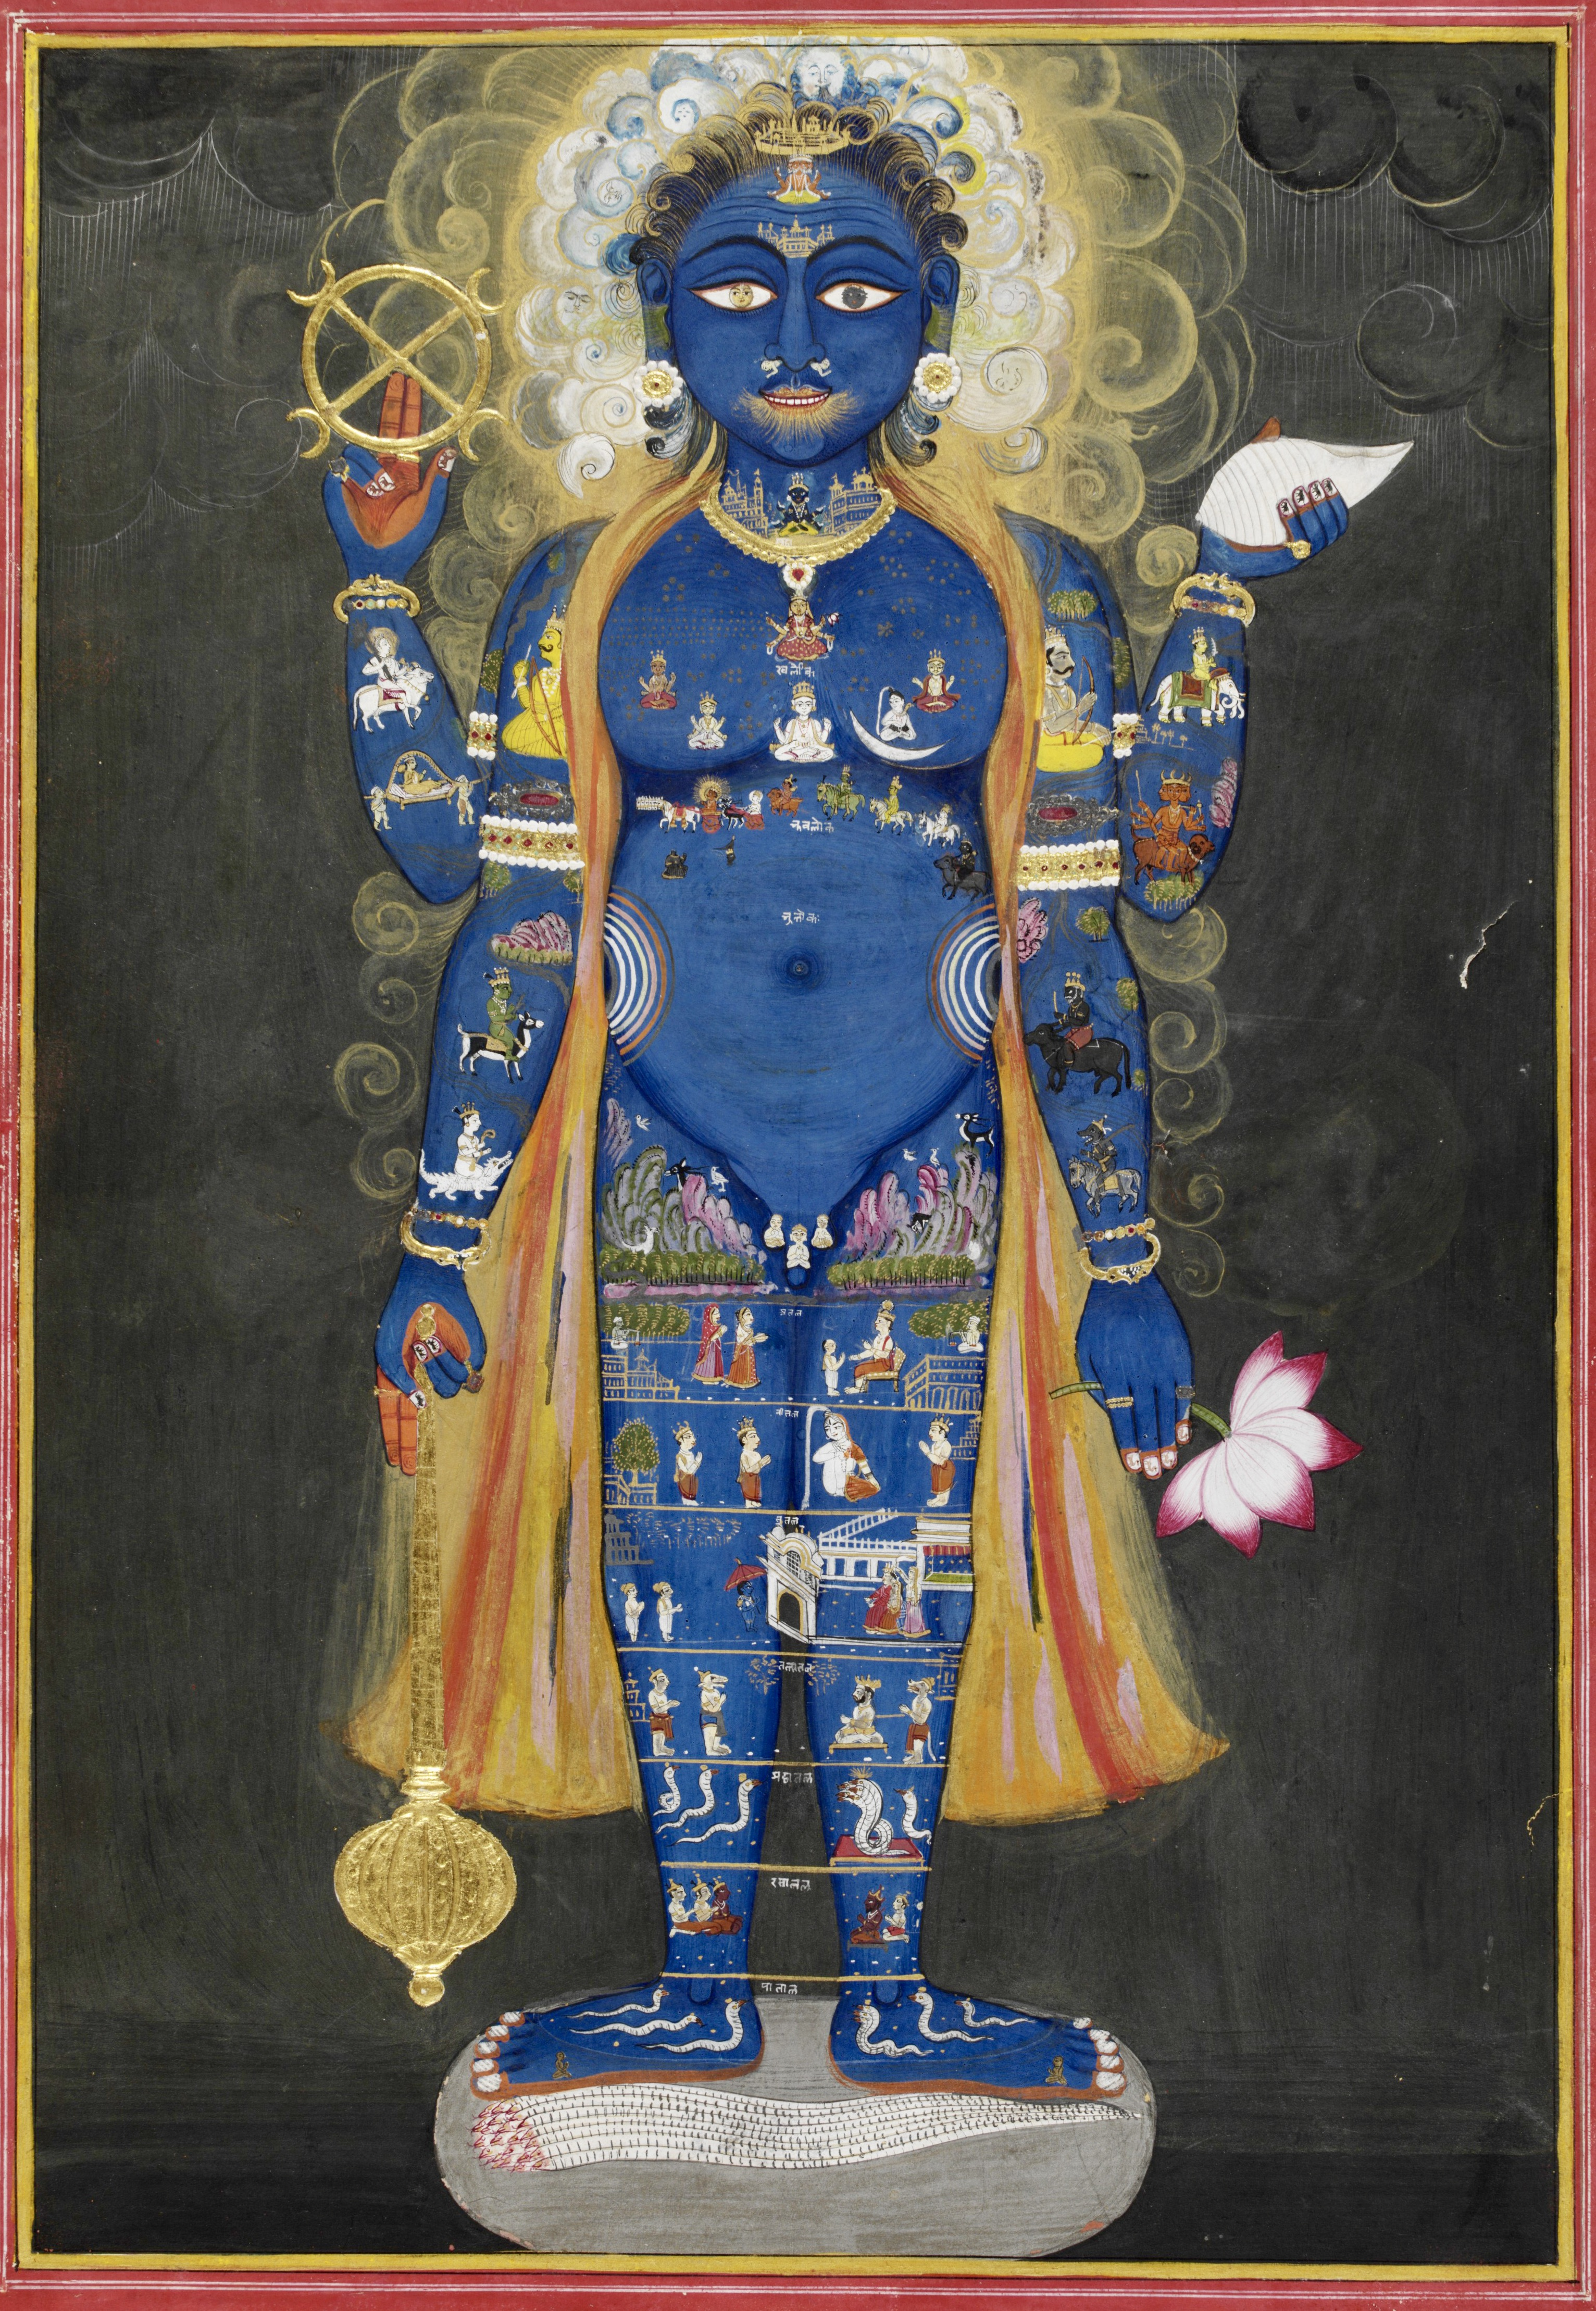
\includegraphics[width=1\textwidth]{pics/Vishnu_Vishvarupa_cropped.jpg}
	\caption{Viṣṇu Viśvarūpa, India, Rajasthan, Jaipur, ca. 1800–1820, Opaque watercolor and gold on paper, 38.5 × 28 cm, Victoria and Albert Museum, London, Given by Mrs. Gerald Clark.}
	\label{fig1}
      \end{figure}
\clearpage
  \begin{figure}[ht]
	\centering
  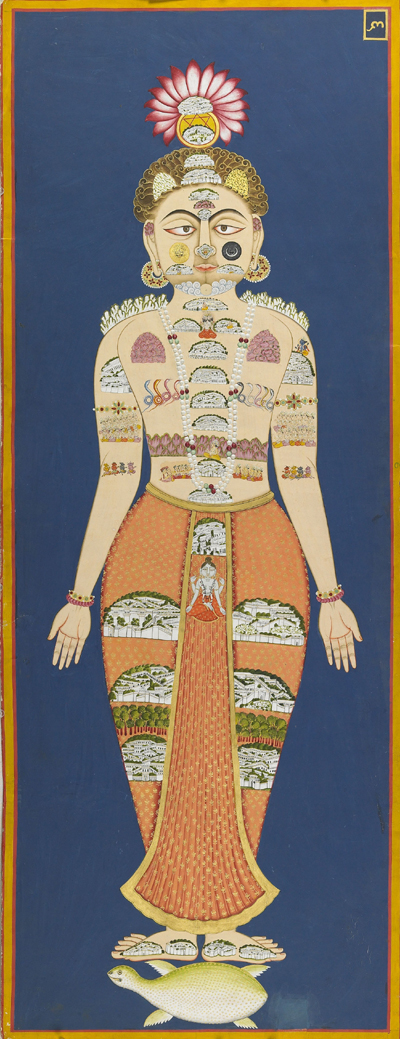
\includegraphics[width=0.5\textwidth]{pics/The_Equivalence_of_Self_and_Universe_(detail),_folio_6_from_the_Siddha_Siddhanta_Paddhati,_(Bulaki),_1824_(Samvat_1881);_122_x_46_cm._Mehrangarh_Museum_Trust..jpg}
	\caption{The Equivalence of Self and Universe (detail), folio 6 from the \textit{Siddhasiddhāntapaddhati} (Bulaki), India, Rajasthan, Jodhpur, 1824 (Samvat 1881), 122 x 46 cm, RJS 2378, Mehragarh Museum Trust.}
	\label{fig2}
      \end{figure}
      % \end{landscape}


\chapter{Bibliography}
 \label{sec:bibli}
   \clearpage
\newpage 
\thispagestyle{empty}
\quad  \addtocounter{page}{-1}

\printbibliography[heading=subbibintoc, title=Consulted Manuscripts, keyword=codex]

\printbibliography[heading=subbibintoc, title=Printed Editions, keyword=printsource]

\printbibliography[heading=subbibintoc, title=Secondary Literature, keyword=seclit]

\printbibliography[heading=subbibintoc, title=Online Sources, keyword=onlinesource]

\end{document}
